\documentclass[11pt, floatsintext]{apa6}
\usepackage{amssymb}
\usepackage{graphicx}
\usepackage[outdir=./]{epstopdf}
%\DeclareGraphicsExtensions{.eps}
\usepackage{caption}
\captionsetup{font=footnotesize}

\usepackage{mathtools}
\usepackage{enumerate}
\usepackage{textcomp}
\usepackage{lingmacros}
\usepackage[draft]{hyperref}
\usepackage{apacite}
\usepackage{listings}
\usepackage{multirow}
\usepackage{stfloats}
\usepackage{todonotes}
\usepackage{svg}
\usepackage{booktabs}
\usepackage{stmaryrd}

\synctex=1
\usepackage{soul}

\newcommand{\den}[1]{\ensuremath{\llbracket #1 \rrbracket}}

\newcommand{\KL}[2]{\ensuremath{D_{KL}({#1}\, \| \, {#2})}}
\newcommand{\E}[2]{\ensuremath{\mathbb{E}_{#1}\left [#2 \right]}}

\newenvironment{figurehere}
	{\def\@captype{figure}}
	{}

\usepackage{lipsum}
%\pagenumbering{gobble}
%\usepackage{apacite}

\linespread{1}


\DeclareGraphicsRule{.tif}{png}{.png}{`convert #1 `dirname #1`/`basename #1 .tif`.png}
\graphicspath{{./figures/}}
 
 \definecolor{Green}{RGB}{10,200,100}
  \definecolor{Red}{RGB}{200,100,50}
\newcommand{\tlg}[1]{\textcolor{Green}{[tom: #1]}}  
\newcommand{\rdh}[1]{\textcolor{Red}{[rdh: #1]}}  


\makeatother

\title{From partners to populations: \\[.1em] A hierarchical Bayesian account of coordination and convention}
\shorttitle{Conventions}
\author{Various people}
\affiliation{Various Universities}

\abstract{Abstract TBD}

\keywords{Keywords TBD}

\authornote{This report is based in part on work presented at the 39th, 40th, and 42nd Conferences of the Cognitive Science Society \cite{hawkins_convention-formation_2017,hawkins_emerging_abstractions_2018,hawkins2020generalizing}. Correspondence should be addressed to Robert D. Hawkins, e-mail: rdhawkins@princeton.edu}

\begin{document}
\maketitle

\begin{quote}
%The speaker wants to be understood [...] %, so he intends to speak in such a way that he will be interpreted in a certain way. 
\emph{In order to judge how he will be interpreted, [the speaker] uses his starting theory of interpretation. % interpreter’s readiness to interpret along certain lines. %Central to this picture is what the speaker believes is 
%The speaker does not necessarily speak in such a way as to prompt the interpreter to apply this prior theory; he may deliberately dispose the interpreter to modify his prior theory. But the speaker’s view of the interpreter’s prior theory is not irrelevant to what he says, nor to what he means by his words; it is an important part of what he has to go on if he wants to be understood.
As speaker and interpreter talk, their ``prior'' theories become more alike; so do their ``passing'' theories. 
%The asymptote of agreement and understanding is when passing theories coincide. 
%But the passing theory cannot in general correspond to an interpreter’s linguistic competence. 
Not only does it have its changing list of proper names and gerrymandered vocabulary, but it includes every successful use of any other word or phrase, no matter how far out of the ordinary [...] 
%Every deviation from ordinary usage, as long as it is agreed on for the moment [...] is in the passing theory as a feature of what the words mean on that occasion. 
Such meanings, transient though they may be, are literal. \\-- \citeA{davidson_nice_1986}.}

\end{quote}

\input{Introduction}

\section{Convention formation as\\ Hierarchical Bayesian inference}


In this section, we propose a unified computational account of \emph{ad hoc} coordination and convention formation that addresses these three empirical puzzles. 
We begin from first principles: What is the core computational problem that must be solved to achieve successful communication?
Classically, this problem has been formulated in terms of coding and compression \cite{Shannon48}. 
An intended meaning in the speaker's mind must be encoded as a signal that is recoverable by the receiver after passing through a noisy transmission channel.
This literal transmission problem has since been enriched to account for \emph{pragmatics} -- the ability of speakers and listeners to use context and social knowledge to draw inferences beyond the literal meaning of messages \cite{sperber1986relevance}.
We take the Rational Speech Act framework \cite<RSA;>{frank_predicting_2012,goodman_pragmatic_2016,FrankeJager16_ProbabilisticPragmatics} as representative of this current synthesis, formalizing communication as recursive social inference in a probabilistic model.
In the next section, we will review this basic framework and then raise two fundamental computational problems facing this framework that motivate our proposal.

\subsection{RSA models of communication with static meaning}

In our referential communication setting\footnote{For concreteness, we restrict our scope to reference in a discrete context of objects, but the same formulation applies to more general spaces of meanings.}, the RSA framework defines a pragmatic speaker, denoted by $S_1$, who must choose an utterance $u$ that will allow their partner to choose a particular target object $o$ from the current communicative context $\mathcal{C}$:
They attempt to satisfy the Gricean Maxims \cite{Grice75_LogicConversation} by selecting utterances proportional to a utility function $U(u;o)$ that balances informativity to an imagined listener against the cost of producing an utterance:
\begin{align}
S_1(u | o) & \propto   \exp\{\alpha_S \cdot U(u; o)\}\label{eq:RSAspeaker} \\
U(u; o) & = (1-w_C) \cdot \underbrace{\log L_0(o | u)}_{\mathclap{\text{informativity}}} -\, w_C \cdot \underbrace{c(u)}_{\mathclap{\text{cost}}} \nonumber 
\end{align}
where $c(u)$ is a function giving the cost of producing $u$, assuming a longer utterances are more costly.
The speaker has two free parameters: $w_C \in [0,1]$ controls the relative weight of informativity and parsimony in the speaker's production, and $\alpha_S \in[0,\infty]$ controls their softmax optimality (i.e. as $\alpha_S \rightarrow \infty$, the speaker increasingly chooses the utterance with maximal utility.)

The imagined \emph{literal listener} $L_0$ in Eq.~\ref{eq:RSAspeaker} is assumed to identify the target using a lexical meaning function $\mathcal{L}(u,o)$ capturing the literal semantics of the utterance $u$.
That is, the probability of the literal listener choosing object $o$ is proportional to the meaning of $u$ under a static lexical meaning function $\mathcal{L}$:
\begin{align}
L_0(o | u) &\propto  \mathcal{L}(u,o)\nonumber
\end{align}
Throughout this paper, we will take $\mathcal{L}$ to be a traditional truth-conditional function evaluating whether a given object is in the extension of the utterance\footnote{Note that the normalization constant may be exactly zero for some possible lexicons -- for instance, if a given utterance is literally false of all objects in context -- in which case these distributions are not well-defined. See Appendix A for technical details of how we address this problem.}:
$$
\mathcal{L}(u,o) = \left\{ \begin{array} {rl} 1 & \textrm{if $o \in \den{u}$} \\ 0 & \textrm{otherwise} \end{array}\right.
$$
However, there are many alternative representational choices compatible with our core model, including fuzzier, continuous semantics \cite{degen2020redundancy} or vector embeddings learned by a neural network \cite[see Appendix B for examples]{potts2019case}, which may be more appropriate for scaling the model to larger spaces of words and referents.
We return to these possibilities in the General Discussion.

%Finally, we may then define a pragmatic listener $L_1$ that inverts their own internal model of an imagined speaker, inferring which intended referent $o\in\mathcal{C}$ would best explain the speaker's choice of utterance $u$:
%\begin{align}
%L_1(o | u) \propto   \exp\{w_L \cdot \log S_1(u | o)\}\nonumber
%\end{align}
%Intuitively, this listener is able to account for alternative utterances the speaker could have chosen to produce.
%For example, if an alternative utterance $u'$ would have perfectly referred to some object $o$, then the fact that the speaker did \emph{not} choose to say $u'$ suggests $o$ is not the intended referent. 

\subsection{Two fundamental problems for static meaning}

This basic framework and its extensions have accounted for a variety of important phenomena in pragmatic language use \cite<e.g.>{Scontras_problang,KaoWuBergenGoodman14_NonliteralNumberWords,TesslerGoodman16_Generics,LassiterGoodman15_AdjectivalVagueness}.
Yet it retains a key assumption from classical models: that the speaker and listener must share the same literal ``protocol'' $\mathcal{L}$ for encoding and decoding messages.
In this section, we highlight two under-appreciated challenges of communication that complicate this assumption. 

The first challenge is \emph{variability} in linguistic meaning throughout a language community. 
Different listeners may recover systematically different meanings from the same message, and different speakers may encode the same message in different ways.
For example, doctors may fluently communicate with one another about medical conditions using specialized terminology that is meaningless to a patient. 
The words may not be in the patient's lexicon, and even common words may be used in non-standard ways.
That is, being fluent speakers of the same language does not ensure perfect overlap for the relevant meanings that need to be transmitted in every context: different partners may simply be using different functions $\mathcal{L}$.

The second challenge is the \emph{non-stationarity} of the world. 
Agents are continually presented with new thoughts, feelings, and entities, which they may not already have efficient conventions to talk about.
For example, when new technology is developed, the community of developers and early adopters must find ways of referring to the new concepts they are working on (e.g. \emph{e-mailing}, \emph{the Internet}). 
Or, when researchers design a new experiment with multiple conditions, they must find ways of talking about their own \emph{ad hoc} abstractions, often converging on idiosyncratic names that can be used seamlessly in meetings.
That is, any literal protocol $\mathcal{L}$ that we may write down at one time would be quickly outdated at a later time \cite<see>[for a demonstration of the related problems posed by non-stationary for large neural language models]{lazaridou2021pitfalls}.
We must have some ability to extend our language on the fly as needed.

\subsection{A hierarchical model of dynamic meaning}

%The model we present in this section aims to provide an explanation for how agents may  these fundamental problems.
Rather than assuming a monolithic, universally shared language, we argue that agents solve the core problems posed by variability and non-stationarity by attempting to continually, adaptively \emph{infer} the system of meaning used by their partner in context.
When all agents are continually learning in this way, we will show that they are not only able to locally coordinate on \emph{ad hoc} meanings with specific partners but also able to abstract away linguistic conventions that are expected to be shared across an entire community.
We introduce our model in three steps, corresponding to three core capacities: hierarchical uncertainty about meaning, online partner-specific learning, and inductive generalization.

\paragraph{C1:~Hierarchical uncertainty about meaning} 

When an agent encounters a communication partner, they must call upon some representation about what they expect different signals will mean to that partner. 
We therefore replace the static function $\mathcal{L}$ with a \emph{parameterized family} of lexical meaning functions by $\mathcal{L}_{\phi}$, where different values of $\phi$ yield different possible systems of meaning. 
To expose the dependence on a fixed system of meaning, Eq.~\ref{eq:RSAspeaker} can be re-written to give behavior under a fixed value of $\phi$:
\begin{align}
L_0(o | u, \phi) &\propto  \mathcal{L}_\phi(u,o)\hfill\label{eq:RSA} \\
U(u; o, \phi) & = (1-w_C) \cdot \log L_0(o | u, \phi) -\, w_C \cdot c(u) \nonumber  \\
S_1(u | o,\phi) & \propto   \exp\{\alpha_S \cdot U(u; o, \phi)\} \nonumber 
%L_1(o | u,\phi) & \propto   \exp\{w_L \cdot \log S_1(u | o, \phi) \nonumber \}
\end{align}
While we will remain agnostic for now to the exact functional form of $\mathcal{L}_\phi$ and the exact parameter space of $\phi$ (see \emph{Inference details} section below), there are two key computational desiderata we emphasize.
First, given the challenge of variability raised in the previous section, these expectations ought to be sensitive to the overall statistics of the population. 
An agent should know that there is tighter consensus about the meaning of \emph{dog} than the meaning of, say, specialized medical terms like \emph{sclerotic aorta} \cite{Clark98_CommunalLexicons}, and conversely, should expect more consensus around how to refer to familiar concepts than new or ambiguous concepts.
Second, this representation should also, in principle, be sensitive to the social identity of the partner: a cardiologist should have different expectations about a long-time colleague than a new patient.

\begin{figure}[t!]
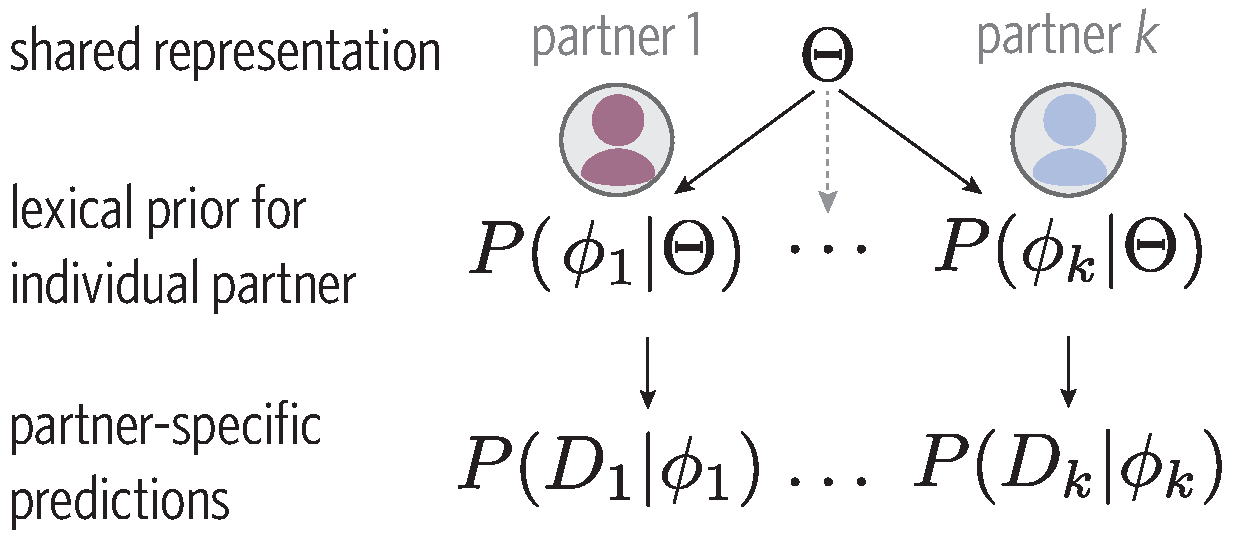
\includegraphics[scale=0.4]{./figures/task1_model.pdf}
\vspace{.5em}
\caption{\emph{Schematic of hierarchical Bayesian model.} At the highest level, denoted by $\Theta$, is a representation of aspects of meanings expected to be shared across all partners. These \emph{global} conventions serve as a prior for the systems of meanings used by specific partners, $\phi_k$. These partner-specific representations give rise in turn to predictions about their language use $P(D_k|\phi_k)$, where $D_k$ represents observations in a communicative interaction with partner $k$. By inverting this model, agents can adapt to \emph{local} partner-specific conventions and update their beliefs about global conventions.}
\label{fig:model_schematic}
\end{figure}
The first desideratum, representing population variability, motivates a \emph{probabilistic} formulation.
Instead of holding a single static function $\mathcal{L}_{\phi}$, which an agent assumes is shared perfectly in common ground (i.e. one $\phi$ for the whole population), we assume each agent maintains \emph{uncertainty} over the exact meaning of words as used by different partners.
In a Bayesian framework, this uncertainty is specified by a prior probability distribution over possible values of $\phi$.
For example, imagine that under some possible values of $\phi$, the term ``sclerotic aorta'' has truth conditions related to a specific condition of the heart, but under other values of $\phi$, it does not: a well-trained doctor approaching a stranger should not assume their partner is using either $\phi$ but should assign some probability to each case.
The introduction of uncertainty over a partner's literal semantics has previously been explored in the context of one-shot pragmatic reasoning, where it was termed \emph{lexical uncertainty} \cite{bergen_pragmatic_2016}, and in the context of iterated dyadic interactions \cite{SmithGoodmanFrank13_RecursivePragmaticReasoningNIPS}. 


The second desideratum, sensitivity to partner-specific meanings, motivates a \emph{hierarchical} model, where uncertainty is represented by a multi-level prior. 
At the highest level of the hierarchy is \emph{community-level} uncertainty $P(\Theta)$, where $\Theta$ represents an abstract ``overhypothesis" about the overall distribution of possible partners. 
$\Theta$ then parameterizes the agent's \emph{partner-specific} uncertainty $P(\phi_{k} | \Theta)$, where $\phi_k$ represents the specific system of meaning used by partner $k$ (see Fig. \ref{fig:model_schematic}). 
We focus for simplicity on this basic two-layer hierarchy, but the model can be straightforwardly extended to representing uncertainty at intermediate layers of social structure, including whether partners belong to distinct sub-communities (e.g. represented by discrete latent variables) or varying along latent dimensions (e.g. represented by a topic mixture). 
We return to these possible extensions in the General Discussion.

To integrate this lexical uncertainty into our speaker and listener models, we assume they each act in a way that is expected to be successful \emph{on average}, under likely values of $\phi_k$ \cite{SmithGoodmanFrank13_RecursivePragmaticReasoningNIPS}.
In other words, they sample actions by marginalizing over their own beliefs $P_S(\phi_k)$ or $P_L(\phi_k)$ about different meanings their partner $k$ may be using.
\begin{align}
L(o|u) &\propto   \exp\left\{\alpha_L \textstyle{\int} P_L(\phi_k)  \log S_1(u|o, \phi_k)\,\,d\phi_k\right\}\nonumber\\
S(u|o) &\propto  \exp\left\{\alpha_S \textstyle{\int} P_S(\phi_k)  U(u; o, \phi_k) \,\,d\phi_k\right\}\label{eq:marginalized}
\end{align}
where $\alpha_S, \alpha_L \in[0,\infty]$ control the speaker's and listener's soft-max optimality, respectively\footnote{We denote $L$ and $S$ without a subscript because they are the only speaker and listener models we use in simulations throughout the paper -- the subscripted definitions are internal constructs used to define these models -- but in the terminology of the RSA framework they represent $L_1$- and $S_1$-level pragmatic agents with lexical uncertainty. We found that higher levels of recursion were not strictly necessary to derive the phenomena of interest, but $L_n$ and $S_n$-level lexical uncertainty models may be generalized by replacing $S_1$ in the listener equation, and $L_0$ in the speaker's utility definition, with standard RSA definitions of $n-1$-level agents \cite<e.g.>{zaslavsky2020rate}.}.

\paragraph{C2: Partner-specific online learning}

The formulation in Eq.~\ref{eq:marginalized} derives how agents ought to act under uncertainty about the lexicon being used by their partner, $P(\phi_k)$.
But how do beliefs about their partner change over time?
Although an agent may begin with significant uncertainty about the system of meaning their partner is using in the current context, further interactions provide useful information for reducing that uncertainty and therefore improving the success of communication.
In other words, \emph{ad hoc} convention formation may be re-cast as an inference problem.
Given observations $D_k$ from interactions with partner $k$, an agent can update their beliefs about their partner's latent system of meaning following Bayes rule:
\begin{equation}
\begin{array}{rcl}
\label{eq:joint_inference}
P(\phi_k, \Theta | D_k)  & \propto &  P(D_k | \phi_k, \Theta) P(\phi_k, \Theta) \\
                           & =   & P(D_k | \phi_k) P(\phi_k | \Theta) P(\Theta)
\end{array}
\end{equation}
This joint inference decomposes the partner-specific learning problem into two terms, a prior term $P(\phi_k | \Theta)P(\Theta)$ and a likelihood term $P(D_k | \phi_k)$.
The prior term captures the idea that, in the absence of strong evidence of partner-specific language use, the agent ought to regularize toward their background knowledge of conventions: the aspects of meaning that all partners are expected to share in common.
The likelihood term represents predictions about how a partner would use language in context under different underlying systems of meaning (as specified in the \emph{Referential Feedback} section below).

Importantly, the posterior obtained in Eq.~\ref{eq:joint_inference} allows agents to explicitly maintain \emph{partner-specific expectations}, as used in Eq.~\ref{eq:marginalized}, by marginalizing over community-level uncertainty:
\begin{equation}
P(\phi_k | D_k) =  \int_{\Theta}P(\phi_k, \Theta | D_k)  d\Theta
\end{equation}
This posterior can be viewed as the ``idiolect'' that has been fine-tuned to account for partner-specific common ground from previous interactions.
We will show that when agents learn about their partner in this way, and adjust their own production or comprehension accordingly (i.e.~Eq.~\ref{eq:marginalized}), they are able to coordinate on stable \emph{ad hoc} conventions.

\paragraph{C3: Inductive generalization to new partners}

The posterior in Eq.~\ref{eq:joint_inference} also provides an inductive pathway for partner-specific data to inform beliefs about community-wide conventions.
Agents update their beliefs about $\Theta$, using data accumulated from different partners, by marginalizing over beliefs about specific partners:
\begin{equation}
\begin{split}
    P(\Theta | D)  = & \int_{\phi} P(\phi, \Theta | D) d\phi \\
%                     \propto & P(\Theta) \int_{\phi} P(D_k | \phi_k) P(\phi_k | \Theta) d\phi
\end{split}
\end{equation}
where $D = \bigcup_{k=1}^N D_k$, $\phi = \phi_1 \times \dots \times \phi_N$, and $N$ is the number of partners previous encountered. 
Intuitively, when multiple partners are inferred to use similar systems of meaning, beliefs about $\Theta$ shift to represent this abstracted knowledge: it becomes more likely that a novel partner in one's community will share it as well.
Note that this population-level posterior over $\Theta$ not only represents what the agent has learned about the central tendency of the group's conventions, but also the \emph{spread} or variability, capturing the notion that some word meanings may be more widespread than others.

The updated $\Theta$ should be used to guide the prior expectations an agent brings into a subsequent interactions with strangers.
This transfer is sometimes referred to as ``sharing of strength'' or ``partial pooling'' because pooled data is smoothly integrated with domain-specific knowledge.
This property has been key to explaining how the human mind solves a range of other difficult inductive problems in the domains of concept learning \cite{KempPerforsTenenbaum07_HBM, tenenbaum_how_2011}, causal learning \cite{KempPerforsTenenbaum07_HBM,KempGoodmanTenenbaum10_LearningToLearn},  motor control \cite{berniker2008estimating}, and speech perception \cite{kleinschmidt2015robust}.
A key consequence of such transfer hierarchical models is the ``blessing of abstraction,'' \cite{GoodmanUllmanTenenbaum11_TheoryOfCausality} where it is possible under certain conditions for beliefs about the community's conventions \emph{in general} to outpace beliefs about the idiosyncracies of individual partners \cite{gershman2017blessing}.
We return to this property in the context of language acquisition in the General Discussion.

\subsection{Further challenges for convention formation}

The formulation in the previous section presents the core of our theory.
Here, we highlight several additional features of our model, which address more specific challenges raised by prior work on communication and which we will encounter in the simulations reported in the remainder of the paper. 
Our organization of these details is motivated by \citeA{spike_minimal_2017}, which recently distilled three common problems that all accounts of convention must address: (1) the availability of referential feedback, (2) a form of information loss or forgetting, and (3) a systemic bias against ambiguity.
Finally, we explain practical details of how we perform inference in this model. 

\paragraph{Referential feedback}

Learning and adaptation depends on the availability and quality of observations $D_k$ throughout a communicative interaction.
If the speaker has no way of assessing the listener's understanding, or if the listener has no way of comparing their interpretation against the speakers intentions, however indirectly, they can only continue to rely on their prior, with no ground for conventions to form  \cite{KraussWeinheimer66_Tangrams,HupetChantraine92_CollaborationOrRepitition,GarrodFayLeeOberlanderMacLeod07_GraphicalSymbolSystems}.
So, what data $D_k$ should each agent use to update their beliefs at a particular point in an interaction?

In principle, we expect that $D_k$ reflects all relevant sources of information that may expose an agent's understanding or misunderstanding, including verbal and non-verbal backchannels (\emph{mmhmm}, nodding), clarification questions, and actions taken in the world.
In the more minimal setting of a reference game, we use the full feedback provided by the task, where the speaker's intended target and the listener's response are revealed at the end of each trial. 
Formally, this information can be written as a set of tuples $D_k = \{o^*, u', o'\}_{t=1}^T$, where $o^*$ denotes the speaker's intended target, $u'$ denotes the utterance they produced, and $o'$ denotes the listener's response, on each previous trial $t$.

Now, to specify the likelihoods in Eq.~\ref{eq:joint_inference} for our referential setting, we assume each agent should infer their partner's lexicon $\phi_k$ by conditioning on their \emph{partner's} previous choices.
The listener on a given trial should use the probability that a speaker would produce $u$ to refer to the target $o^*$ under different $\phi_k$, i.e. $P_L(\{o^*, u', o'\}_t\, | \, \phi_k) = S_1(u'_t \,|\, o^*_t, \phi_k)$, and the speaker should likewise use the probability that their partner would produce response $o'$ after hearing utterance $u$, $P_S(\{o^*, u', o'\}_t \,|\, \phi_k) = L_0(o'_t \,|\, u'_t)$,
This symmetry, where each agent is attempting to learn from the other's behavior, creates a clear coordination problem\footnote{In some settings, agents in one role may be expected to take on more of the burden of adaptation, leading to an asymmetric division of labor \cite<e.g.>{MorenoBaggio14_AsymmetrySignaling}. This may be especially relevant in the presence of asymmetries in power, status, or capability. In principle, this could be reflected in differing values of parameters $\alpha_S$ and $\alpha_L$, but we leave consideration of such asymmetries for future work.}.
In the case of an error, where the agent in the listener role hears the utterance $u'$ and chooses an object $o'$ other than the intended target $o^*$, they will receive feedback about the intended target and subsequently condition on the fact that the speaker chose $u'$ to convey that target.
Meanwhile, the agent in the speaker role will subsequently condition on the likelihood that the listener chose the object $o'$ upon hearing their utterance.
In other words, each agent will subsequently condition on slightly different data leading to conflicting beliefs.
Whether or not agents are able to resolve early misunderstandings through further interaction and eventually reach consensus depends on a number of factors.

\paragraph{Memory and forgetting}

One important factor is imposed by the basis cognitive mechanisms of memory and forgetting.
It is unrealistic to expect that memories of every example of every past interaction in the set of observations $D$ is equally accessible to the agent.
Furthermore, this may be to the agent's advantage.
Without any mechanism for forgetting, early errors may prevent coordination much later in an interaction, as each agent's lexical beliefs must explain all previous observations equally.
Without the ability to discount earlier data points, agents may be prevented from ever reaching consensus with their partner \cite{spike_minimal_2017}.

Forgetting is typically incorporated into Bayesian models with a decay term in the likelihood function \cite{anderson2000adaptive,angela2009sequential,fudenberg2014recency,kalm2018visual}.
$$P(D_k | \phi_k) = \prod_{\tau=0}^T \beta^{\tau} P(\{o^*,u',o'\}_{T-\tau}\, |\, \phi_k)$$
where $\tau=0$ indexes the most recent trial $T$ and decay increases further back through time.
This decay term is motivated by the empirical power function of forgetting \cite{wixted1991form}, and can be interpreted as the expectation over a process where observations have some probability of dropping out of memory at each time step.
Indeed, this likelihood can be derived by simply extending our hierarchical model down an additional layer \emph{within} each partner to allow for the possibility that they are using slightly different lexicons at different points in time; assuming a degree of auto-correlation between neighboring time points yields this form of discounting.
Alternatively, at the algorithmic level, decay can be viewed as a form of weighted importance sampling, where more recent observations are preferentially sampled \cite{pearl2010online}.
While this simple decay model is sufficient for our simulations, we discuss several extensions in the General Discussion that better capture the complexity of memory processes.

\paragraph{Bias against ambiguity}

A third specific challenge is posed by ambiguity: if a speaker uses a label to refer to one target, it is consistent with the data for the listener to subsequently believe that the same expression may be acceptable for other targets as well. 
%How do agents overcome this ambiguity to converge on an \emph{informative} communication system?
In our account, this problem is naturally solved by the principles of \textit{pragmatic reasoning} instantiated in the RSA framework \cite{Grice75_LogicConversation}, which has been explicitly linked to \emph{mutual exclusivity} in word learning \cite{bloom2002children,FrankGoodmanTenenbaum09_Wurwur,SmithGoodmanFrank13_RecursivePragmaticReasoningNIPS,gulordava2020one,ohmerreinforcement}.
Gricean pragmatic reasoning critically allows agents to learn from the \emph{absence} of evidence by reasoning about alternatives. 

Pragmatic reasoning plays two distinct roles in our model.
First, Gricean agents assume that their partner is using language in a cooperative manner and account for this when inferring their partner's language model.
That is, we use these equations as the linking function in the likelihood $P(D_k | \phi_k)$, representing an agent's prediction about how a partner with meaning function $\phi_k$ would actually behave in context (Eq.~\ref{eq:joint_inference}). 
$S_1$ is used to learn from observations generated in the speaker role and $L_1$ is used to learn from observations generated in the listener role.
For example, upon hearing their partner use a particular utterance $u$ to refer to an object $o$, a pragmatic agent can not only infer that $u$ means $o$ in their partner's lexicon, but also that all other utterances $u'$ likely do \emph{not} mean $o$: if they did, the speaker would have used them instead.
Second, agents do not only make passive inferences from observation, they participate in the interaction by \emph{using language} themselves.
A Gricean agent's own production and comprehension is also guided by cooperative principles (Eq.~\ref{eq:marginalized}).

Many minor variations on the basic RSA model have been explored in previous work, and it is worth highlighting three technical choices in our formulation.
First, both agents are ``action-oriented,'' in the sense that they behave proportional to the utility of different actions, according to a soft-max normalization $\sigma(U(z)) = e^{U(z)}/\sum e^{U(z)}$.
This contrasts with some RSA applications, where the listener is instead assumed to be ``belief-oriented,'' simply inferring the speaker's intended meaning without producing any action of their own \cite{qing2015variations}.
Second, our instantiation of lexical uncertainty differs subtly from the one used by \citeA{bergen_pragmatic_2016}, which placed the integral over lexical uncertainty at a \emph{single} level of recursion (specifically, within a pragmatic listener agent).
Instead, we argue that it is more natural in an interactive, multi-agent setting for each agent to maintain uncertainty at the highest level, such that each agent is reasoning about their \emph{partner}'s lexicon regardless of what role they are currently playing.

Lastly, we must define how the $L_0$ agent behaves when an utterance is false of all objects in context under their lexicon (i.e. when the normalization constant is exactly 0). 
Previous proposals have assumed that the $L_0$ should choose uniformly in this case.
However, this assumption has the unintuitive consequence that $S_1$'s utility of using an utterance known to be false of the target may be the same as an utterance known to be true.
To address this concern, we always add a low-prior-probability `null object' to the $L_0$'s context, for which all utterances evaluate to true.
This alternative can be interpreted as a `failure to refer' and effectively prevents $L_0$ from assigning belief to a referent for which the utterance is literally false (this case is distinct from the case of a \emph{contradiction}, which arises when defining the meaning of multi-word utterances in Section \textbf{P1} below.)
See Appendix A for further details and discussion of our RSA implementation.

\paragraph{Inference details}

While our simulations in the remainder of the paper each address different scenarios, we have aimed to hold as many details as possible constant throughout the paper.
First, we must be concrete about the space of possible lexicons that parameterizes the lexical meaning function, $\mathcal{L}_{\phi}$.
For consistency with previous Bayesian models of word learning \cite<e.g.>{XuTenenbaum07_WordLearningBayesian} we take the space of possible meanings for an utterance to be the set of nodes in a concept taxonomy.
When targets of reference are conceptually distinct, as typically assumed in signaling games, the target space of utterance meanings reduces to the discrete space of individual objects, i.e.~$\den{u}_{\phi} = \phi(u) \in \mathcal{O}$ for all $u\in\mathcal{U}$.
For this special case, the parameter space contains exactly $|\mathcal{O}| \times |\mathcal{U}|$ possible values for $\phi$, corresponding to all possible mappings between utterances and individual objects. 
Each possible lexicon can therefore be written as a binary matrix where the rows correspond to utterances, and each row contains one object.
The truth-conditional function $\mathcal{L}_{\phi}(u,o)$ then simply checks whether the element in row $u$ matches object $o$.
For example, there are four possible lexicons for two utterances and two objects:
$$\phi \in \left\{\begin{bmatrix}
\bluesquare \\
\orangecircle \\
\end{bmatrix},
\begin{bmatrix}
\orangecircle \\
\bluesquare \\
\end{bmatrix},
\begin{bmatrix}
\orangecircle\\
\orangecircle \\
\end{bmatrix},
\begin{bmatrix}
\bluesquare  \\
\bluesquare \\
\end{bmatrix}\right\}$$

Second, having defined the support of the parameter $\phi$, we can then define a simplicity prior $P(\phi) \propto \exp\{-|\phi|\}$ following \citeA{FrankGoodmanTenenbaum09_Wurwur}, where $|\phi|$ is the total size of each word's extension, summed across words in the vocabulary. 
Again, for traditional signaling games, this reduces to a uniform prior because all possible lexicons are the same size: $\phi(u_i) \sim \textrm{Unif}(\mathcal{O})$.
We can compactly write distributions over $\phi$ in terms of the same utterance-object matrix, where row $i$ represents the marginal distribution over possible meanings of utterance $u_i$.
For example, the uninformative prior for two utterances and two objects can be written:
$$P(\phi) =  \begin{array}{ccc}
& & \bluesquare \,\,\,\,\,\,\orangecircle \\
\begin{bmatrix}
\textrm{Unif}\{\bluesquare,\orangecircle\} \\
\textrm{Unif}\{\bluesquare,\orangecircle\} \\
\end{bmatrix} & = & \begin{bmatrix}
.5 & .5  \\
.5 & .5 \\
\end{bmatrix}
\end{array}$$
This prior becomes more important for \textbf{P3}, however, where we consider spaces of referents with more complex conceptual structure and a larger space of possible meanings. 
A single word may apply to multiple conceptually related referents or, conversely, may have an empty meaning, where it is effectively removed from the agent's vocabulary.
In this more general case, a simplicity prior generically favors smaller word meanings as well as a smaller effective vocabulary size, since the null meaning has the smallest extension. 

Finally, while the probabilistic model we have formulated in this section is theoretically well-motivated and mathematically well-defined, it has previously been challenging to actually derive predictions from it.
Historically, interactive models have been challenging to study with closed-form analytical techniques and computationally expensive to study through simulation, likely contributing to the prevalence of simplified heuristics in prior work. 
Our work has been facilitated by recent advances in probabilistic inference techniques that have helped to overcome these obstacles. 
We have implemented our simulations in the probabilistic programming language WebPPL \cite{GoodmanStuhlmuller14_DIPPL}.
All of our simulations iterate the following trial-level loop: (1) sample an utterance from the speaker agent's distribution, given the target object, (2) sample an object from the listener's object distribution, given the utterance sampled in the previous step, (3) append the results to the list of observations, and (4) update both agents' posterior distributions, conditioning on these observations before continuing to the next trial.

To obtain the speaker and listener distributions (steps 1-2; Eq.~\ref{eq:RSA}), we always use exhaustive enumeration for exact inference.
We would prefer to use enumeration to obtain posteriors over lexical meanings as well (step 4; Eq.~\ref{eq:joint_inference}), but as the space of possible lexicons $\phi$ grows, enumeration becomes intractable.
For simulations related to \textbf{P2} and \textbf{P3}, we therefore switch to Markov Chain Monte Carlo (MCMC) methods to obtain samples from each agent's posteriors, and approximate the expectations in Eq.~\ref{eq:marginalized} by summing over these samples. 
Because we are emphasizing a set of phenomena where our model makes qualitatively different predictions than previous models, our goal in this paper is to illustrate and evaluate these \emph{qualitative} predictions rather than provide exact quantitative fits to empirical data.
As such, we proceed by examining predictions for a regime of parameter values ($w_S, w_L, w_C,\beta$) that help distinguish our predictions from other accounts, and leave the more computationally expensive task of empirical parameter estimation to future studies.


\section{Phenomenon \#1: \\ Increasing efficiency in ad hoc convention formation}


%If our lexical priors -- our global conventions -- serve as a source of stability in meaning over longer timescales, then what accounts for our extraordinary flexibility  over short timescales? How do we coordinate on efficient local conventions, or \emph{conceptual pacts}, for talking about things we've never talked about before? In this section, we review the dynamics of coordination within repeated reference games and explore the possibility, formalized in Chapter 2, that rapid adaptation can be understood in a Bayesian modeling framework as lexical inference given partner-specific data.%: $P(\mathcal{L}_i | D_i, \Theta)$. 

When we first encounter a new communication partner in a new context, we call upon some representation about what we think different signals mean to them. 
In our account, this representation is given by $P(\Theta)$, the global background prior.
While we are agnostic to the exact function parameterized by $\Theta$, there are two properties that our account emphasizes.
First, this representation of meaning must be sensitive to the overall statistics of the population: there is more consensus about the meaning of \emph{dog} than the meaning of \emph{sclerotic aorta} in the general population. 
Second, this representation should also, in principle, be sensitive to the identity of the partner: a cardiologist should have different expectations about a new colleague than a new patient.

The most well-known phenomenon in repeated reference games is a reduction in message length over multiple rounds \citeA{KraussWeinheimer64_ReferencePhrases, ClarkWilkesGibbs86_ReferringCollaborative}. 
The first time participants referred to a figure, they tend to use a lengthy, detailed description (``the upside-down martini glass in a wire stand'') but with a small number of repetitions -- between 3 to 6 times, depending on the pair -- the description is reduced down to the limit of just one or two words (``martini''). 
These final messages are as short or shorter than the messages participants choose for \emph{themselves} in the future  \citeA{FussellKrauss89_IntendedAudienceCommonGround} and are often incomprehensible to overhearers who were not present for the initial messages \cite{SchoberClark89_Overhearers}.
These observations set up the central empirical puzzle of convention formation: how does a short word or phrase that would have been completely ineffective for communicating under the initial lexical prior become perfectly understandable over mere minutes of interaction? What changes inside participants' minds in the interim? 

One simple non-social explanation --- that reduction is merely an effect of familiarity or repetition on the part of the speaker --- can be easily dispelled. 
When participants are asked to repeatedly refer to the same targets for a hypothetical partner, no reduction is found, and in some cases utterances actually get longer \cite{HupetChantraine92_CollaborationOrRepitition}. 
Whatever is changing must be a result of the \emph{interaction} between partners.
An alternative explanation suggested by our probabilistic model is that reduction is driven by \emph{ad hoc} word learning as communication partners coordinate on names. 
If long initial messages can be explained as the result of initial uncertainty in the lexical prior, as discussed in the previous section, then a decrease in uncertainty may license shorter messages.

There is some evidence supporting this alternative explanation in prior empirical work.
For example, \citeA{BrennanClark96_ConceptualPactsConversation} counted \emph{hedges} across repetitions.
Hedges are expressions like \emph{sort of} or \emph{like}, and morphemes like \emph{-ish}, that explicitly mark uncertainty or provisionality, such as \emph{a car, sort of silvery purple colored} \cite{BrennanClark96_ConceptualPactsConversation,Fraser10_Hedging,MedlockBriscoe07_HedgeClassification}.
If participants reduce their lexical uncertainty over successive rounds, then we might expect a corresponding decrease in explicit markers of this uncertainty. 
Indeed, \citeA{BrennanClark96_ConceptualPactsConversation} found a much greater occurrence of hedges on the first round than the final round (26\% and 2\%, respectively).
Additionally, very few hedges were found on early trials in less ambiguous contexts (e.g. referring to a shoe in the context of dogs and fish), lending support for the specific use of hedges to mark uncertainty rather than a generic social use when first beginning to talk with a new partner.

\subsection{Model simulations}

\begin{figure*}
\centering
    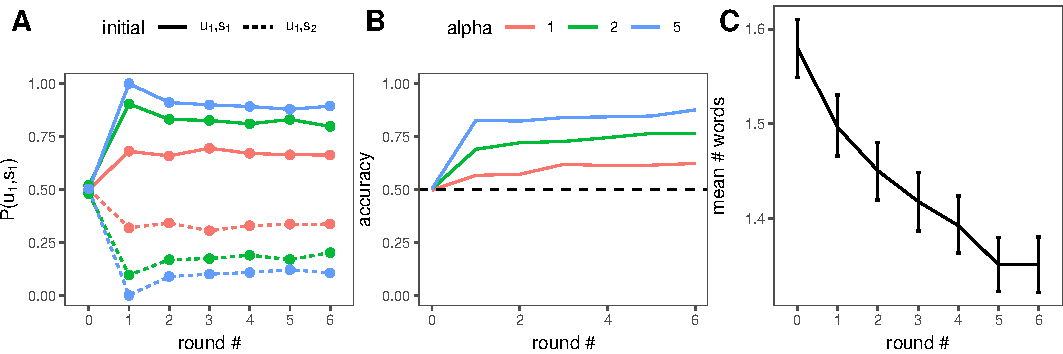
\includegraphics[scale=.9]{sec1-modelResults.pdf}
  \caption{Schematic of model}
  \label{fig:sec1model}
\end{figure*}


In this section, we show that the mechanism of uncertainty reduction is sufficient to produce reduction in utterance length across repeated interaction.

\paragraph{Simulation 1.1: Coordination}

First, we show how agents updating their meaning functions in this way can coordinate even in the absence of strong initial priors. 
The initial choices in an interaction can be taken as evidence for a particular lexicon and become the basis for successful communication, even when both speaker and listener are uncertain at the beginning.
As a simple test case, consider an environment with two objects ($\{o_1, o_2\}$), where the speaker must choose between two utterances ($\{u_1, u_2\}$) with equal production costs. 
For the prior $P(\mathcal{L})$ over the meaning of each utterance, we define a Beta distribution\footnote{In our implementation, we use exact enumeration over coarse-grained bins; experiments using variational inference on the full continuous distribution give similar results}, so on the first round both utterances are equally likely to apply to either shape. 
If the speaker were trying to get their partner to pick $o_1$, then because each utterance is equally (un)informative, they could only randomly sample one (say, $u_1$), and observe the listener's selection of a shape (say, $o_1$, a correct response). 
On the next round, the speaker uses the observed pair $\{u_1, o_1\}$ to update their beliefs about their partner's true lexicon, uses these beliefs to generate a new utterance, and so on. 
To examine expected dynamics over multiple rounds, we forward sample many possible trajectories.

We observe several important qualitative effects in our simulations. 
First, and more fundamentally, the evidence that a knowledgeable listener responded to utterance $u$ by choosing a particular object $o$ provides support for lexicons in which $u$ is a good fit for $o$. 
Hence, the likelihood of the speaker using $u$ to refer to $o$ will increase on subsequent rounds (see Fig.\ref{fig:sec1model}A). 
In other words, the initial symmetry between the meanings can be broken by initial random choices, leading to completely arbitrary but stable mappings in future rounds. 

Second, because the listener is updating their meaning representation from the same observations under the same set of assumptions, both partners converge on a \emph{shared} set of meanings; hence, the expected accuracy of selecting the target object rises on future rounds (see Fig. \ref{fig:sec1model}B). 
Third, because one's partner is assumed to be pragmatic via recursive Rational Speech Act mechanisms, agents can also learn about \emph{unheard} utterances. 
Observing $d = \{(u_1, o_1)\}$ also provides evidence that $u_2$ is \emph{not} a good fit for $o_1$.
This effect arises from Gricean maxims: if $u_2$ were a better fit for $o_1$, the speaker would have used it instead \cite{Grice75_LogicConversation}. 
Fourth, \emph{failed references} can lead to conventions just as effectively as successful references: if the speaker intends $o_1$ and says $u_1$, but then the listener incorrectly picks $o_2$, the speaker will take this as evidence that $u_1$ actually means $o_2$ in their partner's lexicon and become increasingly likely to use it that way on subsequent rounds.

\paragraph{Simulation 1.2: Reduction}

Next, we show how our model explains reduction of utterance length over multiple interactions. 
For utterances to be reduced, of course, they must vary in length, so we extend our grammar to include \emph{conjunctions}. 
Conjunctions are one of the simplest ways to construct longer, non-atomic utterances compositionally from lexical primitives, using the product rule \cite<see also>[who instead consider negation]{SteinertThrelkeld16_CompositionalSignaling}:
$$\mathcal{L}(u_i \textrm{ and } u_j, o) = \mathcal{L}(u_i, o) \times \mathcal{L}(u_j, o)$$
We consider a scenario where two objects $\{o_1, o_2\}$ differ along two different features. 
The speaker thus has four primitive words at their disposal -- two words for the first feature ($\{u_{11}, u_{12}\}$) and two for the second $\{u_{21}, u_{22}\}$. 
While we established in the previous section that conventions can emerge over a reference game in the complete absence of initial preferences, players often bring such preferences to the table. 
A player who hears `ice skater' on the first round of a tangrams task is more likely to select some objects more than others, even though they still have some uncertainty over its meaning in the context. 
To show that our model can accommodate this fact, we allow the speaker's initial prior meanings to be slightly biased. 
We assume $u_{11}$ and $u_{21}$ are a priori more likely to mean $o_1$ and $u_{12}$ and $u_{22}$ are more likely to mean $o_2$.

We ran 1000 forward samples of 6 rounds of speaker-listener interaction, and averaged over the utterance length at each round \footnote{In our simulations, we used $\alpha = 10$ but found the basic reduction effect over a range of different biases}. 
Our results are shown in Figure \ref{fig:sec1model}C: the expected utterance length decreases systematically over each round. 
To illustrate in more detail how this dynamic is driven by an initial rational preference for redundancy relaxing as reference becomes more reliable, we walk step-by-step through a single trajectory. 
Consider a speaker who wants to refer to object $o_1$. 
They believe their knowledgeable partner is slightly more likely to interpret their language using a lexicon in which $u_{11}$ and $u_{12}$ apply to this object, due to their initial bias. 
However, there is still a reasonable chance that one or the other alone actually refers more strongly to $o_2$ in the true lexicon. 
Thus, it is useful to produce the conjunction "$u_{11}$ and $u_{12}$" to hedge against this possibility, despite its higher cost. 
Upon observing the listener's response (say, $o_1$), the evidence is indeterminate about the separate meanings of $u_{11}$ and $u_{12}$ but both become increasingly likely to refer to $o_1$. 
In the trade-off between informativity and cost, the shorter utterances remain probable options. 
Once the speaker chooses one of them, the symmetry collapses and that utterance remains most probable in future rounds. 
In this way, meaningful sub-phrases are omitted over time as the speaker becomes more confident about the true lexicon. 

\paragraph{Model comparison}

Here we compare this model to several simpler baselines to establish which components of the model are necessary and sufficient for the desired behavior.

\rdh{e.g., no pragmatics, pragmatics only in learning rule or only in decision rule instead of both, simpler pragmatics (reasoning about $L_0$ instead of $L_1$), point estimate instead of uncertainty, effect of different parameter regimes.} 

\rdh{It may also be useful to explicitly show that the simpler Roth-Erev RL updating from this literature doesn't reduce, or even better show that this kind of simpler update rule is equivalent to something within our framework as a point estimate representation with maximum likelihood or something...?}

%In the limit, it doesn't matter whether you have pragmatics in both learning rule or decision rule. 
%In case where it's only in production rule, you'll produce the data with the necessary biases in learning.



\subsection{Discussion}

Our model contrasts in several ways with prior theories of adaptation in language use. 
First, we contrast the mechanisms in our model with the lower-level priming mechanisms proposed in the influential \emph{interactive alignment} account \cite{pickering2004toward, pickering2006alignment, garrod2009joint}.
We fully expect that these low-level priming effects are at play in repeated reference tasks --- they are inescapable in any memory-based retrieval process.
However, the gradual reduction of the speaker's utterance length is not obviously primed by any features of the listener's language use; indeed, it happens even when the listener is prevented from saying anything at all and only feedback about the listener's accuracy is provided. 
Explaining why speakers think they can get away with shorter descriptions given sparse evidence of understanding (e.g. a correct response or a simple gesture of confirmation) and resort to longer descriptions given evidence of misunderstanding (e.g. an incorrect response) requires a mechanism for semantic coordination in the absence of lower-level statistics.

Second, we consider agent-based models implementing simple update rules \cite{steels_self-organizing_1995,barr_establishing_2004,young_evolution_2015}.
These models all share some mechanism that makes utterances more likely to be produced after communicative successes and less likely after communicative failures.
It is not clear why agents using such rules would initially prefer to produce longer utterance without some notion of uncertainty, or how naively reinforcing initially long descriptions could lead to reduction without some mechanism for \emph{credit assignment} to the component words.
It is plausible that using more sophisticated reinforcement schemes -- for instance, neural network architectures incorporating compositionality and recurrence into production \cite<e.g>{lazaridou2018emergence} -- could predict patterns of reduction with the addition of a cost term, but such a scheme would be much closer to our meta-learning approach, implemented using gradient-based learning \cite{hawkins2019continual}.

Our simulations in this section are also consistent with recent analyses of exactly \emph{what} gets reduced \cite{hawkins2020characterizing}.
Is the speaker adopting a fragment shorthand by randomly and noisily dropping words, or are they simplifying or narrowing their descriptions to names by systematically omitting redundant details?
Closed-class parts of speech like determiners and prepositions \emph{are} much more likely to be dropped than open-class parts of speech like adjectives and nouns, and entire modifying clauses are more likely to be dropped together than expected by random corruption.
This accords with early hand-tagged analyses by \citeA{Carroll80_NamingHedges}, which found that in three-quarters of transcripts from \citeA{KraussWeinheimer64_ReferencePhrases} the short names that participants converged upon were prominent in some syntactic construction at the beginning, often as a head noun that was initially modified or qualified by other information. 
These more fine-grained analyses suggest that reduction is grounded in the prior lexical content of the interaction and the speaker's increasing confidence in how the listener will interpret an initially ambiguous label. 



\section{Phenomenon \#2: \\Ad hoc conventions are shaped by context}

%!TEX root = ../dissertation.tex
%\begin{savequote}[75mm]
%\qauthor{Quoteauthor Lastname}
%\end{savequote}

%% Set up problem
\begin{figure*}[t]
\begin{center}
{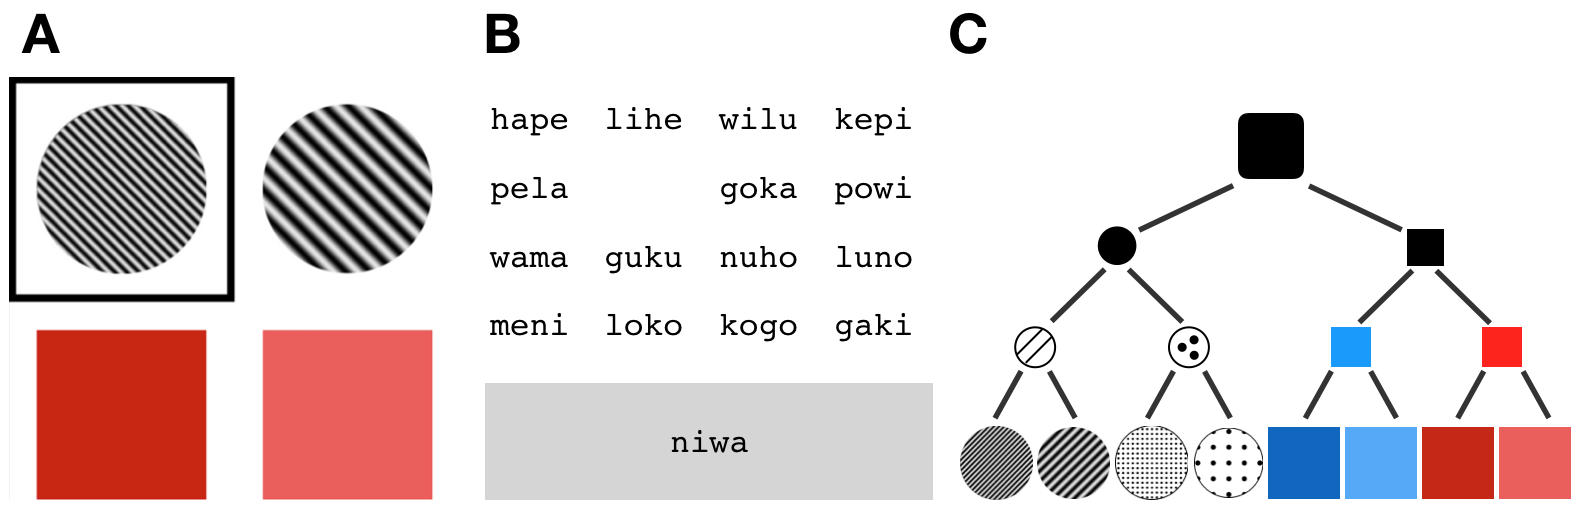
\includegraphics[scale=.63]{./figures/Sec2-design.png}}
{\caption{{\emph{Domain for context-sensitivity.} (A) Example of \emph{fine} context where one of the distractors belongs to the same fine-grained branch of the hierarchy as the target (i.e.\ another striped circle), so any abstract label would be insufficient to disambiguate them. The target is highlighted for the speaker with a black square. (B) Drag-and-drop chat box interface. (C) Hierarchical organization of stimuli.\label{fig:context_design}}}}
\vspace{-2ex}
\end{center}
\end{figure*}

In the previous section, we examined a mechanism for rapid, partner-specific learning that allows agents to form stable but arbitrary \emph{ad hoc} conventions. 
Here, we show how our model also accounts for key patterns of \emph{context-sensitivity} as arising naturally from communicative need in dyadic interaction.
For example, while most English speakers have the basic-level word ``tree'' in their lexicon, along with a handful of subordinate-level words like ``maple'' or ``fir,'' we typically do not have labels exclusively referring to each individual tree in our yards.
If we need to refer to a specific tree, we instead create a referring expression \emph{on the fly} (e.g. ``the one with the bright red leaves close to the street'').
Meanwhile, we \emph{do} often have conventionalized labels (i.e. proper nouns) for individual people and places that we regularly encounter in our daily lives.
Why do conventions form at some levels of abstraction rather than others?

We hypothesize that local context shapes conventions through the mechanisms of pragmatic inference over the shorter timescales of dyadic interactions.
When a particular partner uses a label to refer to an object in a context, we can infer that they do not believe it applies to the distractors as well; otherwise, they would have known it would be confusing and chosen a different label.
First, we fill a gap in the empirical literature by collecting a new dataset of artificial-language repeated reference games manipulating context, allowing us to observe the emergence of \emph{ad hoc} conventions in the absence of global priors.
%This experiment manipulates the context of distractors in a repeated reference game where participants must interactively coordinate on an artificial language from scratch. 
Second, we show that context-sensitivity naturally emerges from our inferential account, via recursive pragmatic reasoning in the likelihood term agents use throughout coordination.
In both the empirical data and our model simulations, we find that conventions come to reflect the distinctions that are functionally relevant for communicative success. 
Furthermore, we find that pragmatic reasoning is needed for these effects to arise. 

%Suppose, mixing thought experiments from \citeA{Wittgenstein09_PhilosophicalInvestigations} and \citeA{Quine13_WordAndObject}, that two travelers meet in a forest, with no language in common. One is cooking dinner, and the other agrees to help in exchange for food and shelter. What kind of micro-language do they coordinate on to solve this joint task, and how is it shaped by context? 
			
\subsection{Experimental methods}

\subsubsection{Participants}

We recruited 278 participants from Amazon Mechanical Turk to play an interactive, multi-player game using the framework described in \citeA{Hawkins15_RealTimeWebExperiments}. Pairs were randomly assigned to one of three different conditions, yielding $n=36$ dyads in the \emph{course} condition, $n=38$ in the \emph{fine} condition, and $n=53$ in the \emph{mixed} condition after excluding participants who disconnected before completion.\footnote{Planned sample sizes, exclusion criteria, and behavioral analysis plan were pre-registered at \url{https://osf.io/2hkjc/}. All statistical tests in mixed-effects models reported in this section use degrees of freedom based on the Satterthwaite approximation \cite{luke2017evaluating}.}

\subsubsection{Procedure \& Stimuli}
Participants were paired over the web and placed in a shared environment containing an array of objects (Fig.\ \ref{fig:context_design}A) and a `chatbox' to send messages from a randomly generated vocabulary (Fig.\ \ref{fig:context_design}B). On each of 96 trials, one player (the `speaker') was privately shown a highlighted target object and allowed to send a single word to communicate the identity of this object to their partner (the `listener'), who subsequently made a selection from the array. Players were given full feedback, swapped roles each trial, and both received bonus payment for each correct response.

The objects that served as referents were designed to cluster in a fixed three-level hierarchy with shape at the top-most level, color/texture at the intermediate levels, and frequency/intensity at the finest levels (see Fig.\ \ref{fig:context_design}C). Each communicative context contained four objects. Distractors could differ from the target at various level of the hierarchy, creating different types of contexts defined by the finest distinction that had to be drawn. We focus on two: \emph{fine} trials, where the closest distractor belongs to the same fine-grained subordinate category (e.g.\ another striped circle; see Fig.\ \ref{fig:context_design}A), and \emph{coarse} trials, where the closest distractor belongs to a coarser level of the conceptual hierarchy (e.g.\ dotted circle instead of striped circle).\footnote{Even coarser trials with super-ordinate distractors (e.g.\ a circle target among three square distractors) were logically possible but would have introduced several experimental confounds; we opted to leave these trial types out of our design and conduct the minimal manipulation.} Fixed arrays of 16 utterances (enough to allow the potential for full expressibility) were randomly generated for each pair (and held constant across trials) by stringing together consonant-vowel pairs into pronounceable 2-syllable words (see Fig.\ \ref{fig:context_design}B).

Critically, we manipulated the statistics of the context in a between-subjects design to test the context-sensitivity of conventions. 
In the \emph{fine} condition, all targets appeared in fine contexts; in the \emph{course} condition, all targets appeared in course contexts; and in the \emph{mixed} condition, half of the targets appeared in each context.
Sequences of trials were constructed by randomly shuffling targets and trial types within blocks and ensuring no target appeared more than once in a row. 
In addition to behavioral responses collected over the course of the game, we designed a post-test to explicitly probe players' final lexica. For all sixteen words, we asked players to select all objects that a word can refer to (if any), and for each object, we asked players to select all words that can refer to it (if any). 
This bidirectional measure allows us to check the internal validity of the lexica reported.

%\begin{figure}[t]
%\begin{center}
%{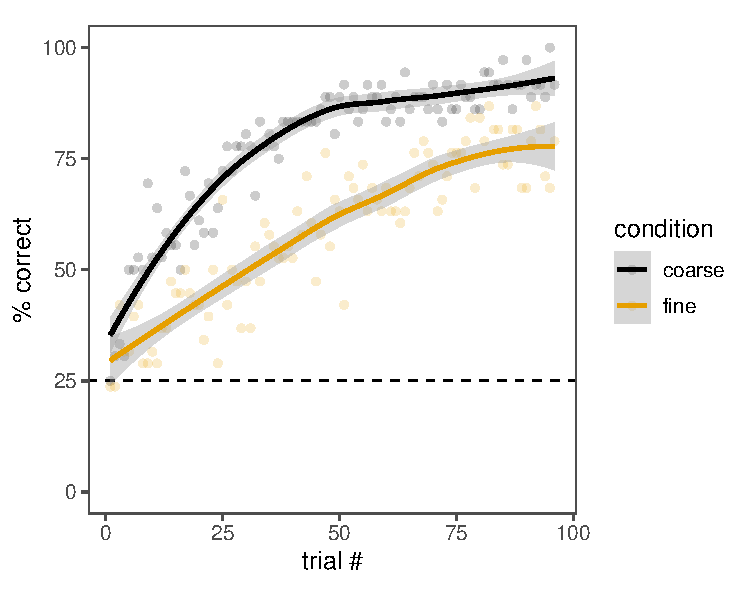
\includegraphics[scale=1]{./figures/sec2_empirical_accuracy.pdf}}
%{\caption{{
%\label{fig:context_accuracy}}}}
%\vspace{-3ex}
%\end{center}
%\end{figure}

\begin{figure}[t]
\begin{center}
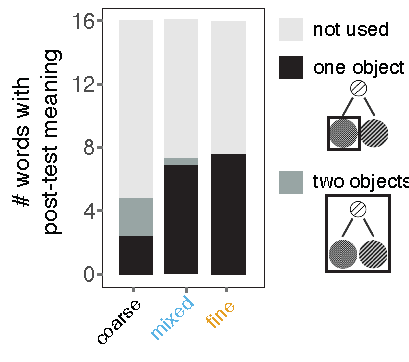
\includegraphics[scale=1]{./figures/Exp2_postTest}
\caption{\emph{Different lexicons emerge in different contexts.} Mean number of words, out of a word bank of 16 words, that human participants reported giving specific meanings (black; applying to 1 object) or abstract meanings (dark grey; applying to 2 objects).}
\label{fig:sec2postTest}
\end{center}
\end{figure}


\subsection{Behavioral results}

\paragraph{Partners successfully learn to communicate}

Although participants in all conditions began with no common basis for label meanings, performing near chance on the first trial (proportion correct $= 0.19$, 95\%~CI~$=~[0.13, 0.27]$), most pairs were nonetheless able to coordinate on a successful communication system over repeated interaction (see Fig.\ \ref{fig:context_accuracy}). 
A mixed-effects logistic regression on listener responses with trial number as a fixed effect, and including by-pair random slopes and intercepts, showed a significant improvement in accuracy overall, $z = 14.4, p < 0.001$. 
Accuracy also differed significantly \emph{across} conditions (Fig.\ \ref{fig:context_accuracy}): adding an additional main effect of condition to our logistic model provided a significantly better fit, $\chi^2(2) = 10.8, p = 0.004$. 
Qualitatively, the \emph{coarse} condition was easiest for participants, the \emph{fine} condition was hardest, and the \emph{mixed} condition was in between.
Finally, the (log) response time taken by the speaker to choose an utterance also decreased significantly over the course of the game, $t(126) = -19.7, p < 0.001$, from approximately 20 seconds to only 6 seconds on average, indicating that lexical mappings became increasingly established or accessible.

\begin{figure*}[t]
\begin{center}
\includegraphics[scale=0.9]{Sec2-results.pdf}
\vspace{1ex}
\caption{\emph{Comparison of Simulation 2.1 results to empirical data}. (A) Participants in our behavioral experiment learned to coordinate on a successful communication system, but converged faster in the coarse condition than the fine condition. Each point is the mean proportion of correct responses by listeners; curves are nonparametric fits. (B) The number of unique words used by speakers in each repetition block increased in the fine condition but stayed roughly constant in the coarse condition. (C-D) The same metrics computed on the output of Simulation 2.1, qualitatively matching the patterns observed in the empirical data.}
\label{fig:lexiconContent}
\end{center}
\end{figure*}

\paragraph{Partners converge on similar conventions}

Another indicator of successful learning is convergence or alignment of lexica between partners within a dyad. 
Before using post-test responses to compute similarity between partners, however, we examine the internal consistency of an individual's post-test responses. 
For each participant, we counted the number of mismatches between the two directions of the lexicon question (e.g.\ if they clicked the word `mawa' when we showed them one of the blue squares, but failed to click that same blue square when we showed `mawa'). 
In general, participants were quite consistent: out of 128 cells in the lexicon matrix (16 words $\times$ 8 objects), the median number of mismatches was 2 (98\% agreement), though the distribution has a long tail (mean $= 7.3$). 
We therefore conservatively take a participant's final lexicon to be the \emph{intersection} of their word-to-object and object-to-word responses.

Using these estimates of each participant's lexicon, we compute the overlap between partners. 
For most pairs, partners aligned strongly by the end, with a median post-test overlap of 97.6\% (125 out of 128 entries). 
Because these matrices were extremely sparse, however, just a a few mismatches could have a large impact on performance. 
Overall accuracy in the game is strongly correlated with alignment: partners who reported more similar lexica at the end also tended to perform significantly better at the task ($r = 0.77, t(120) = -13.5,~p <0.001$).  
Despite these broad markers of convergence at the group level, individual performance had a long tail: a subpopulation of 29 games (11\% of coarse games, 18\% of mixed games, and 39\% of fine games) still showed relatively poor performance late in the game (see Fig.~\ref{fig:full_accuracy_grid} in Appendix for full histograms).
%For the subsequent analyses focusing on the content of the lexicon, we exclude games with accuracy below the pre-registered criterion of 75\% on the final quarter of trials to ensure we are examining only the content of lexica that converged.
%\rdh{double-check this. add better motivation if I do this.}

\paragraph{Contextual pressures shape the lexicon}

We predicted that in contexts regularly requiring speakers to make fine distinctions among objects at subordinate levels of the hierarchy, we would find lexicalization of specific terms for each object (indeed, a one-to-one mapping may be the most obvious solution in a task with only 8 objects). 
Conversely, when no such distinctions were required, we expected participants to adaptively lexicalize more abstract terms.
One coarse signature of this prediction lies in the \emph{efficiency} of the resulting lexicon: lexicalizing abstract terms should require participants to use fewer terms overall.

To test this prediction, we operationalize vocabulary size as the number of words in each participant's reported lexicon in the post-test (i.e.\ the words for which they marked at least one object in the post-test in an internally consistent way). 
We then conducted a mixed-effects models predicting each individual's vocabulary size as a function of dummy-coded condition factors, with random intercepts for each game. 
We found that participants in the \emph{coarse} condition reported significantly smaller, more efficient lexica ($m = 4.9$ words) than participants in the \emph{mixed} ($m=7.1, t(110.8)=7.6, p < 0.001$) and \emph{fine} condition ($m = 6.9, t(109.3) = 6.4, p < 0.001$; see Fig.\ \ref{fig:lexiconContent}A). 
At the same time, smaller vocabularies did not lead to poorer coverage over objects: the median number of objects where participants agreed on the same word was 7 out of 8 in the \emph{coarse} condition, compared to 6 in the \emph{mixed} condition and 5.5 in the \emph{fine} condition. 
Differences across conditions do not reach significance ($p = 0.4, p = 0.09$, respectively), but may reflect the relative sub-populations of participants who did not fully converge. 

How did these lexica emerge over the course of interaction? 
To measure the effective vocabulary size used throughout the interaction, we considered the total number of unique words produced within each repetition block.
Because all eight objects appeared as the target once in each block, this measure takes a maximum value of 8, in the case where a different word was used for every object, and a minimum value of 1, in the case where the same word was used for every object.
We constructed a mixed-effects regression model predicting the effective vocabulary size, including fixed effects of condition and repetition block, and random intercepts and effects of repetition block for each dyad. 
As in the post-test reports, we found an overall main effect of condition, with participants in the fine condition using significantly fewer words across all repetition blocks: $m = 4.9$ in coarse, compared to $m=5.8, t(124)=6.1, p <0.001,$ in mixed $m=6.8, t(124) =11.4, p < 0.001$).
Critically, however, we also found a significant interaction between the course and fine conditions. 
The effective vocabulary size gradually increased over time in the fine condition but remained roughly constant in the coarse condition, $b = 0.12, t = 4.5, p < 0.001$, see Fig. \ref{fig:lexiconContent}B.
This interaction, where participants initially attempt to reuse the same terms across targets in the fine condition, is consistent with a gradual differentiation based on communicative need.

Finally, if participants in the \emph{coarse} condition could get away with fewer words in their lexicon, what are the meanings of the words they do have? 
We counted the numbers of `specific' terms (e.g.~words that refer to only one object) and `abstract' terms (e.g.~words that refer to two objects) in the post-test. 
We found that the likelihood of lexicalizing abstractions differed systematically across conditions (see Fig.\ \ref{fig:lexiconContent}A). 
Participants in the \emph{coarse} condition reported significantly more abstract terms ($m=2.3$) than in the \emph{fine} ($m = 0.24, t(121.2) = 8.5, p < 0.001$) or \emph{mixed} ($m=0.65, t(122.7)= 7.3, p < 0.001$) conditions, where lexicons contained almost exclusively specific terms.
The modal system in the fine condition was exactly eight specific terms with no abstract terms, and the modal system in the coarse condition was exactly four abstract terms (red, blue, striped, spotted) with no specific terms.
However, even in the coarse condition, many individual participants reported a mixture of terms (see Fig.\ \ref{fig:lexiconContent}C).

\subsection{Model simulations}

Our empirical results show that different communicative contexts systematically lead to different communicative conventions.
Critically, the sequence of targets was held constant across conditions; only the distractors were manipulated.
This task poses several distinct challenges for models of coordination and convention formation.
First, the context constantly changes, with a subset of only four of the eight total objects shown on each trial.
Second, the stimuli are embedded in a conceptual taxonomy, where some objects are more similar than others.
In this section, we show how our model explains such sensitivity as the consequence of pragmatic reasoning \cite<e.g.>{goodman_pragmatic_2016,FrankeJager16_ProbabilisticPragmatics} over a space of taxonomic word meanings.

We evaluate the extent to which local context shapes our agents' conventions through a series of simulations.
For each dyad in our human dataset, we pair up two artificial agents and present them the same stimulus sequence of targets and contexts that human participants saw.
Our artificial agents swapped speaker and listener roles on each trial, as human participants did, and updated their beliefs after each trial using their own history: that is, while we matched the stimulus sequence, the models did not observe human data. 

Again following \citeA{XuTenenbaum07_WordLearningBayesian}, we consider a space of meanings that reflects the conceptual structure of the stimulus hierarchy. 
In addition to 8 meanings at the sub-ordinate level (one for each individual object), we populate the hypothesis space with 4 meanings at the basic-level (striped, spotted, blue, red), 2 meanings at the super-ordinate level (circle and square), 1 exhaustive meaning (shape), and 1 ``null'' meaning, which does not apply to any of the objects.
We populate the utterance space with 8 single-word labels, which simplifies the speaker model: the utterance cost term is constant across all utterances, so it does not have an effect on speaker behavior.
Finally, we will assume a simplicity prior over possible lexicons, $P(\phi) \propto \exp\{|\phi|\}$, where $|\phi|$ is the total size of each word's extension, summed across words in the vocabulary \cite{FrankGoodmanTenenbaum09_Wurwur}.
This simplicity prior over the lexicon space penalizes meanings with larger extensions, so \emph{a priori}, agents have an inductive bias toward subordinate terms.
For ease of presentation, we consider the parameter setting of $w_L=5,w_S=10$ and memory discounting parameter of $\beta = 0.8$.% (see Model comparison below for a more thorough evaluation of these parameters).

\paragraph{Simulation 2.1: Context-sensitivity}

\begin{figure}[t]
\begin{center}
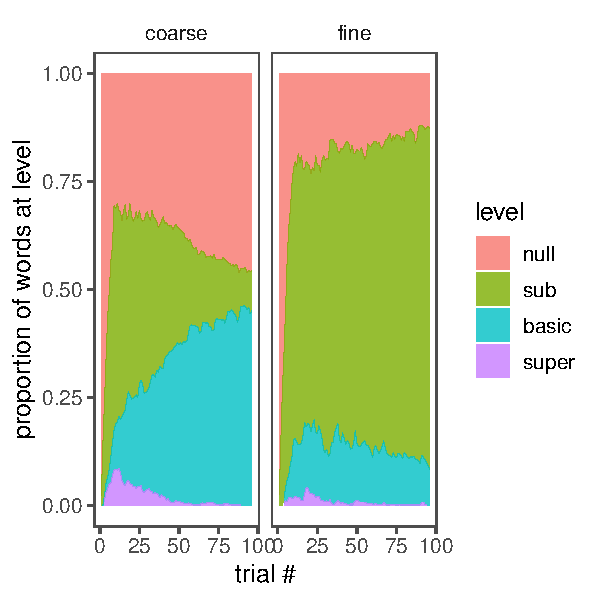
\includegraphics{evolution.pdf}
\caption{\emph{Dynamics of lexical beliefs over time in Simulation 2.1.} Regions represent the average proportion of words at each level of abstraction in an agent's beliefs about the lexicon. In the coarse condition, agents initially assume subordinate terms but gradually abstract away to a smaller number of basic-level terms; in the fine condition, however, agents become more confident of subordinate terms.}
\label{fig:evolution}
\end{center}
\end{figure}

First, we compare the model's learning curves across context conditions (Fig. \ref{fig:sec2model}B). 
We focus on the \emph{coarse} and \emph{fine} conditions for simplicity, since this single comparison captures the core phenomena of interest.
In a mixed-effects logic regression, we find that communicative accuracy steadily improves over time across conditions, $b=0.72, z = 16.9, p<0.001$.
However, we also find a significant interaction with condition: the rate of improvement is significantly higher in the coarse condition than the fine condition, $b=-0.49, z=9.3, p <0.001$. 
These effects track our qualitative findings in the human data: our artificial agents are able to successfully coordinate, but do so more easily in the coarse condition than the fine condition. 

Second, we examine the effective vocabulary sizes that emerge from our simulations. 
We use the same measure of unique words produced in each repetition block that we used in our analyses of human data above. 
In an identical mixed-effects model, we again an overall main effect of condition, with agents in the fine condition using significantly fewer words across all repetition blocks ($m = 4.7$ in \emph{coarse}, $m=6.5$ in \emph{fine,} $t = 4.5, p < 0.001$).
However, we also found a significant interaction: the effective vocabulary size gradually increased over time in the fine condition compared to the coarse condition, $b = 0.18, t = 8.1, p < 0.001$, see Fig.~\ref{fig:sec2model}A.
These effects suggest that the model converges to roughly the same lexicon sizes as humans do.

Finally, we examine more closely the emergence of terms at different levels of abstraction.
We have access not only to the outward behavior of our simulated agents, but also their internal \emph{beliefs} about their partner's lexicon.
So we can not only query these beliefs at the very \emph{end} of the game, as we did in our empirical post-test, we can also directly examine the evolution of these beliefs from the very beginning of the interaction.
At each time point in each game, we take the single meaning with highest probability for each word.

In Fig. \ref{fig:evolution}, we show the proportion of words with meanings at each level of abstraction, collapsing across all games in each condition.
Most critically for comparison with empirical data, we find that the \emph{final} proportion of basic-level vs. subordinate-level terms is significantly different across the coarse and fine conditions.
Only 9\% of words had subordinate-level meanings (green) in the coarse condition, compared with 79\% in the fine condition, $\chi^2(1) = 436, p < 0.001$.
At the same time, 45\% of words had basic-level meanings (blue) in the coarse condition, compared with only 8\% in the fine condition, $\chi^2(1) = 136, p < 0.001$.
The remaining words in each condition were assigned the `null` meaning (red), consistent with an overall smaller effective vocabulary size in the coarse condition.
These effects are consistent with human post-test responses.

What dynamics give rise to these final proportions?
Qualitatively, we observe that agents begin with assumptions of `null' meanings due to their simplicity prior but quickly begin assigning meanings based on their partner's usage.
In both conditions, both basic-level meanings and simpler subordinate-meanings are consistent with the data, with a general preference for simpler meanings.
After the first repetition block, however, agents in the coarse condition begin pruning out some of the subordinate-level terms and become increasingly confident of basic-level meanings and agents in the fine condition become even more confident of subordinate level meanings. 



%\paragraph{Model comparison}

%\rdh{TODO: we need to decide which comparisons are most interesting. may need to implement baseline model from other papers (e.g. Steels-style, or Spike et al. implementation?) for a more explicit comparison to models outside our class of Bayesian agents...}

%We compare our model to (1) a simpler case when both agents condition on the same data (i.e. the true target) even after an unsuccessful communication attempt, and (2) ask what happens when we manipulate forgetting parameter, or remove it?
%
%In a non-pragmatic variant of our model, agents use words proportional to their literal meaning and assume their partner is doing the same. 
%In this case, their lexicon converges to a degenerate 1-word (shape) state.
%Because an initial usage is consistent with all levels of abstraction, one of the agents will eventually extend the same word to different object. 
%Then the only way to subsequently accommodate this extension in the interaction history is to rule out more specific meanings. 
%The non-pragmatic agent has no way of knowing that this degenerate solution is confusing to their partner, and will continue to prefer it because it's literally true of every object.

\subsection{Discussion}

How does context shape conventions? 
There is abundant evidence that languages adapt to the needs of their users, and the context-sensitive emergence of abstractions demonstrated in this section suggests that the driver of this adaptation may lie in the rapid adaptability of agents in individual dyadic interaction. 
By manipulating context statistics in a real-time experiment, we evaluated the extent to which our model captured patterns of context-sensitivity in the behavioral data.

Previous proposals have handled context-sensitivity in different ways.
In some common settings for convention formation, there is no explicit representation of context at all, as in the task known as the ``Naming Game'' where agents coordinate on names for objects in isolation \cite{steels2012experiments,baronchelli2008depth}. 
In other common settings, context is central but held constant throughout interactions, as in Lewis signaling games \cite{lewis_convention:_1969}, where agents use a fixed set of messages to communicate a fixed set of world states \cite{skyrms2010signals,BrunerEtAl14_LewisConventions}.

One of the most sophisticated studies of context in prior work is the Discrimination Game of \citeA{steels2005coordinating}, which examined the joint formation of color categories and color naming conventions.
As in our experiments, contexts were generated randomly on each trial from a large space and stimuli are embedded in a similarity space (with similarity based on Euclidean distance in continuous space rather than taxonomic relations).
Unlike our task, contexts were not systematically manipulated, and the resulting level of abstraction was not evaluated: the only restriction was to ensure that color chips were a fixed minimum distance apart  \cite<see also>[which found that imposing a realistic Just Noticeable Difference function as the minimum distance on communicative contexts leads to human-like color naming systems]{baronchelli2010modeling}.

In models using Roth-Erev reinforcement learning update rules or simple neural networks, the referential context is sometimes accounted for with a \emph{lateral inhibition} heuristic used by both the speaker and listener agents \cite{franke2012bidirectional}.
If communication is successful, the connection strength between the label and object is not only increased, the connection between the label and competing objects (and, similarly, between the object and competing labels) is explicitly \emph{decreased} by a corresponding amount \cite<see also>{steels2005coordinating}.
This lateral inhibition heuristic is functionally similar to our pragmatic reasoning mechanism, in terms of allowing the agent to learn from negative evidence (i.e. the speaker's choice \emph{not} to use a word, or the listener's choice \emph{not} to pick an object). 
Under an inferential framework, however, this property emerges as a natural consequence of well-established Gricean principles of pragmatic reasoning.
Reasoning about a partner's intentions, either while updating beliefs about their lexicon or while selecting an action, naturally instantiates a kind of inductive bias for \emph{mutual exclusivity} \cite{gulordava2020one,ohmerreinforcement,FrankGoodmanTenenbaum09_Wurwur}.

Our results may help to illuminate the relationship between our concepts and words, which are often treated interchangeably. While our mental taxonomies are adaptive to the natural perceptual structure of the world \cite{MervisRosch81_CategorizationReview} %(Rosch et al, 1976; Mervis \& Rosch ,1981; Murphy \& Smith, 1982), 
it is far from inevitable that all levels of these conceptual hierarchies become conventionalized as lexical items. There are many perfectly natural concepts that are not represented by distinct words in the English language: for instance, we do not have words for each tree in our yards, or for ad-hoc concepts %like \emph{things to sell at a garage sale} 
\cite{Barsalou83_AdHocCategories}. Indeed, English speakers are often fascinated by foreign words like the Danish ``hygge'' (a specific notion of coziness) or Scottish ``tartle'' (hesitating when introducing someone because you've forgotten their name) that are difficult to express in English.
Our results highlight communicative needs to distinguish, in context, as a force behind the choice to lexicalize some fine-grained concepts. 
A related direction for future work is to explore the relationship between communicative need and \emph{basic-level} structure.

While we showed how abstract words emerge from efficiency even in a task requiring only reference to individual objects, there are other clear functional advantages to having abstract terms in the lexicon. For one, they allow speakers to efficiently refer to large, potentially infinite, sets of things, and make generalizations about categories, e.g.\ ``Dogs bark'' \cite{TesslerGoodman16_Generics}. Future work should explore this as an additional pressure toward abstract, nested nouns.
Similarly, the option to refer to more specific concepts with compound terms (e.g.~``spotted dog''), which was not available in our experiment, may impact final conventions.
We expect that labels will become lexicalized when the cost incurred by frequently using a compositional construction exceeds the cost of adding an additional word to the lexicon. 
Future work should also explore these hypotheses about how lexicalization of nominal terms trades off with compositionality. 
Our shared lexical conventions are richly structured systems with meanings at multiple levels of abstraction. 
We are constantly supplementing our existing language with local conventions, as we need them.


\section{Phenomenon \#3: \\Generalization to new partners in a social network}

\input{Generalization}

\section{General Discussion}

%!TEX root = ../dissertation.tex
In this paper, we considered the computational challenge faced by agents trying to communicate in a variable and non-stationary landscape of meaning.
We first proposed a hierarchical Bayesian approach to semantic adaption that formalized three broad mechanisms exposed by the prior literature.
%Because theories of adaption have been under-constrained by fine-grained empirical data, we then collected and used recent NLP techniques to analyze a large corpus from a replication of the classic tangrams task.
%Inspired by insights from these analyses, we designed a targeted artificial language experiment to test our hypothesis that context shapes conventions and a graphical communication experiment to test the object- and interaction-specificity of conventions.
We conclude by discussing some broader questions raised by the theoretical perspective we have advanced.

\paragraph{Language acquisition}

We have suggested that the lexical learning mechanisms adults use to coordinate on conventions \emph{within} dyadic interactions may be the same as those supporting language acquisition more broadly.
Our partial pooling model thus suggests a new emphasis on the role of partner-specificity and generalization in development.
Most laboratory tasks investigating cross-situational word learning in children use only use a single speaker \cite{asdf}, and even sophisticated models of cross-situational word learning \cite[e.g.]{FrankGoodmanTenenbaum09_Wurwur} collapse over \emph{who} is talking. 

Yet, as we have argued throughout this work, there is substantial variability across different speakers that poses a challenge for children. 
If the majority of child-directed speech only comes from a single primary caregiver, then the child may face a difficult generalization problem once they begin interacting with others. 
Upon hearing an unfamiliar word from a novel speaker, or a familiar word utterance with an unfamiliar meaning, it could be a quirk of that particular speaker \emph{or} indicative of a globally shared convention. 
There may therefore be substantial path-dependence in acquisition, as children develop their lexical prior and become better attuned to the overall variability in the population \cite<see>[Chap. 6]{Clark09_FirstLanguageAcquisition}. 

This slow-developing lexical prior is one of several explanation for why young children are so terrible at coordinating on local conventions in repeated reference games \cite{GlucksbergKraussWeisberg66_DevoRefGames,KraussGlucksberg77_SocialNonsocialSpeech}. 
When an experimenter feeds them the messages that adult speakers produced naturally, they had no trouble, even as they reduced down to one- or two-word utterances. 
When they played with one another, however,  Kindergardeners continued to make errors even after 15-16 repetitions; children as old as fifth grade only improved with assistance from the experimenter and never approached the perfect levels of adult performance. 
Instead of beginning with the long indefinite descriptions full of hedges and modifiers that adults provide, nursery-school speakers began with short, highly idiosyncratic descriptions like \emph{Mother's dress}. 
If adult speakers' long hedge-filled messages are indeed motivated by lexical uncertainty, then perhaps young children have simply not obtained enough linguistic variability to calibrate their lexical prior. 
Alternatively, if the pragmatic reasoning required to produce informative utterance depends on theory of mind, then the high processing demands of the task may simply be inhibited performance \cite<e.g.>{SetohScottBaillargeon16_FalseBelief}. 

\todo[inline]{do you think it's just that children have not obtained enough linguistic variability, or do you think there is some representational constraint (e.g., lack of repesentational capacity that allows children to use lexical priors that are different from their own, like in a FB-task failure kind of way)?
i guess another way to ask this question is -- are lexical priors essentially representations of others' beliefs, or knowledge/epistemic states? such that the ability to retrieve or use them is constrained by ToM development? or is this a separate thing? at least even infants seem to be sensitive to foreign vs native language speakers, or speaker differences in accents.}

\paragraph{Similarities and differences across communication modalities}

%\begin{quote}
%The oral modality is not well suited to conveying messages mimetically (i.e., iconically), even though that function is also important to human languages. This function is, however, very well served by the manual modality. \cite[p.155]{}
%\end{quote}

While we have focused primarily on verbal and textual communication channels, research on the dynamics of adaptation in other communication modalities, including graphical \cite{GarrodFayLeeOberlanderMacLeod07_GraphicalSymbolSystems,TheisenEtAl10_SystematicityArbitrariness,hawkins2019disentangling} and gestural \cite{FayListerEllisonGoldinMeadow13_GestureBeatsVocalization,bohn2019young} modalities, is important for our account in several ways.
First, it is a core claim of our hierarchical model that the basic cognitive mechanisms underlying adaptation and convention formation are domain-general.
In other words, there is nothing inherently special in our account about spoken or written language as far as our ability to coordinate . 
Any system that we use to communicate should display similar \emph{ad hoc} learning dynamics because in every case, agents are trying to infer the system of meaning being used by their partner.
Directly comparing behavior in repeated reference games across different modalities is therefore necessary to determine which adaptation effects, if any, are robust and attributable to modality-general mechanisms.

Second, at the same time, our hierarchical learning model claims a critical role for the priors we build up across interactions with many individuals.
We therefore predict that different communication modalities should display certain systematic differences due to the representational structure of the communication channel.
For example, in the verbal modality, the tangram shapes from \cite{ClarkWilkesGibbs86_ReferringCollaborative} are highly innominate -- most people do not have much experience naming or describing them with words, so the global prior is weak and local adaptation plays a greater role.
In the graphical modality, where communication takes place by drawing on a shared sketchpad, agents can be expected to have a stronger prior rooted in assumptions about shared perceptual systems and visual similarity \cite{fan2018common} -- drawing a quick sketch of the tangram's outline may suffice for understanding.
Other stimuli have precisely the opposite property: to distinguish between natural images of dogs, agents may have developed strong global conventions in the linguistic modality (e.g. `husky', `poodle', `pug', etc) but drawing the necessary fine distinctions in the graphical modality may be initially very costly for novices, requiring the formation of local conventions. 
Gesture also has its own distinctive prior, which also allows communicators to use time and the space around them to convey mimetic or depictive meanings that may be difficult to encode verbally or graphically \cite{goldin-meadow_role_1999,clark2016depicting,mcneill1992hand}. 

%If we adhered solely to the verbal modality, we would be limited to a fairly narrow range of stimuli (e.g. abstract shapes/tangrams) where behavior in the lab isn't totally dominated by strong prior conventions people bring into the interaction. 
%For example, similar phenomena Pictionary games where participants use a whiteboard to draw messages instead of an auditory or text-based channel \cite{GarrodFayLeeOberlanderMacLeod07_GraphicalSymbolSystems,TheisenEtAl10_SystematicityArbitrariness,hawkins2019disentangling}.

Another modality-based manipulation is to attempt to destroy or scramble any meaningful priors that people might carry into the social interaction.
For example, \citeA{Galantucci05_EmergenceOfCommunication} introduced a novel `seismograph' interface for communication -- a stylus that could be moved side-to-side or lifted up or down to make contact with the sketch pad while the vertical dimension drifted downward at a constant rate.
The resulting messages consequently look nothing like the usual kinds of symbols people create: the relationship between motor actions and perceptual output is broken such that executing a familiar movement for a symbol or numeral instead produces an odd, wavy scribble.
Despite the relative lack of priors on signal meanings in this medium, people were nevertheless able to converge on successful signaling systems in repeated reference games \cite{RobertsGalantucci12_DualityOfPatterning,RobertsEtAl15_IconocityOnCombinatoriality}.
Other novel modalities used in iterated reference games include a `whistle' language where movements along a vertical touch bar slider correspond to changes in pitch \cite{VerhoefRobertsDingemanse15_Iconicity} and a visual analog where movements along the slider were presented visually \cite{VerhoefEtAl16_TemporalLanguage}.
Our model ought to be able to account for production and comprehension across these modalities simply by exchanging its encoder and decoder components to use an appropriate prior.

\paragraph{What is being adapted?}

While we have focused on how participants coordinate on \emph{lexical} meaning, this is only one of many levels at which conventions may form. 
In more complex circumstances, there is often initial uncertainty not just about which of a small set of targets a particular message refers to, but how to represent the relevant targets of reference in the first place. 
Learning to communicate effectively may require discovering a lower-dimensional representation in which the targets of reference vary.
For instance, when using sketches to communicate about the identity of complex pieces of music \cite{HealeySwobodaUmataKing07_GraphicalLanguageGames}, a particular set of strokes could correspond to any number of properties (pitch, tempo, melody, rhythm, intensity) at any temporal granularity. 
This is made particularly clear in a classic maze game \cite{GarrodAnderson87_SayingWhatYouMean}: in order to give effective spatial directions, speakers had well-tuned lexical priors but had to coordinate on what space of \emph{referents} to use (e.g. paths, coordinates, lines, landmarks). 

Prior theories have assumed representations of lexical meanings are relatively fixed and the only learning taking place is how one's partner construes a multi-stable percept. 
For examine, this seems to be what \citeA{BrennanClark96_ConceptualPactsConversation} had in mind when they coined the term \emph{conceptual pact}, and \cite{stolk2016conceptual} have influentially argued that partners in communication construct shared conceptual spaces. 
Given present data it is not clear how these two sources of uncertainty could be teased apart, though certain kinds of conventions (e.g. proper names or acronyms) seem to rely more on binding new linguistic tokens to meanings than on constructing new conceptualizations.
Thus, we expect both levels of coordination are likely to play an important role. 
Our probabilistic model could be extended to handle additional levels of coordination by placing uncertainty over a hyper-parameter corresponding to the intended feature dimension that must be jointly inferred with the correspondence along that dimension. 

\todo[inline]{Cite Hawkins, Kwon, Sadigh, Goodman to argue that gradient-based meta-learning with neural network representation is an alternative architecture that is more computationally tractable at scale than a fully probabilistic model.}

\paragraph{Additional layers of social structure}

Real-world communities are much more complex than the simple networks we considered: each speaker takes part in a number of overlapping subcommunities. 
For example, we use partially distinct conventions depending on whether we are communicating with psychologists, friends from high school, bilinguals, or children \cite{auer_code-switching_2013}.
For instance, when a scientist is talking to other scientists about their work, they know they can use efficient technical shorthand that they would avoid when talking to their non-expert friends and family. 
Previous work has probed representations of community membership by manipulating the extent to which cultural background is shared between speaker and listener.
For example, \citeA{IsaacsClark87_ReferencesExpertsNovices} paired participants who had either lived in NYC or had never been there for a task referring to landmarks in the city (e.g. ``Rockefeller Center''). 
Within just a few utterances from a novel partner, people could infer whether they were playing with an expert or novice and immediately adjust their language use to be appropriate for this inferred identity. 
Social information about a partner’s group can be so important that even players in artificial-language games react to the restrictions of social anonymity by learning to identify members of their community using distinctive signals \cite{roberts_experimental_2010}.

For future work using hierarchical Bayesian models to address the full scale of an individual's  network of communities, additional social knowledge about these communities must be learned and represented in the generative model.
Larger-scale networked experiments can be used to evaluate the hypothesis that a hierarchical representation of conventions includes not just a partner-specific level and population-wide level but also intermediate community levels. 
This hypothesis can be formalized by including additional latent representations of community membership into our hierarchical model.
That is, in addition to updating our model of a particular \emph{partner} based on immediate feedback, even sparse observations of a partner's language use may license much broader inferences about their lexicon via diagnostic information about their social group or background. 
If someone's favorite song is an obscure B-side from an 80s hardcore band, you can make fairly strong inferences about what else they like to listen to and how similar they might be to you \cite{VelezEtAl16_Overlaps, GershmanEtAl17_StructureSocialInfluence}. 
Similarly, if someone casually refers to an obscure New York landmark you also recognize, you can safely update your beliefs about their lexicon to include a number of other conventions shared among New Yorkers. 
Lexica cluster within social groups, so inverting this relationship can yield rapid lexical learning from inferences about social group membership.

\paragraph{Closing thought}

Language is not some rigid body of knowledge that we acquire at an early age and deploy mechanically for the rest of our lives. 
Nor is its evolution a slow, inter-generational drift. 
It is a means for communication -- a shared interface between minds -- and must therefore adapt over the rapid timescales required by communication. 
In other words, we are constantly learning language. 
Not just one language, but a family of related languages, across every repeated interaction with every partner. 




\section{\bf Acknowledgments}
\small

\bibliography{ref}
\bibliographystyle{apacite}

\renewcommand{\thefigure}{A\arabic{figure}}
\renewcommand{\thetable}{A\arabic{table}}
\setcounter{table}{0}
\setcounter{figure}{0}





\begin{table*}[th!]
\centering
\resizebox{\textwidth}{!}{%
\begin{tabular}{@{}lll@{}}
\toprule
\textbf{}                                   & \textbf{Parameter}                                              & \multicolumn{1}{l}{\textbf{Example parameter settings}}                 \\ \midrule
\multirow{11}{*}{\textbf{Partner design}}    & \multirow{3}{*}{What feedback is provided?}                & - no feedback at all                                                  \\
                                            &                                                                 & - only correct/incorrect                                                   \\
                                            &                                                                 & - real-time responses from partner                                         \\ \cmidrule(l){2-3} 
                                            & \multirow{3}{*}{Are you playing with the same partner?}         & - same partner for whole game                                              \\
                                            &                                                                 & - swap out partners every round                                            \\
                                            &                                                                 & - swap after $k$ rounds                                                    \\ \cmidrule(l){2-3} 
                                            & \multirow{3}{*}{What do you know about your partner?}         & - anonymous stranger                                              \\
                                            &                                                                 & - stranger with perceptual information                                            \\
                                            &                                                                 & - close friend                                                    \\ \cmidrule(l){2-3}                                             
                                            & \multirow{2}{*}{How consistent are roles across repetitions?}   & - consistent director/matcher                                              \\
                                            &                                                                 & - alternate roles each round                                               \\ \midrule
\multirow{7}{*}{\textbf{Stimulus design}}   & \multirow{2}{*}{How familiar are targets?}                      & - very familiar: colors, household objects                                 \\
                                            &                                                                 & - not at all familiar: tangrams, novel line drawings                       \\ \cmidrule(l){2-3} 
                                            & \multirow{2}{*}{How complex are targets?}                       & - very complex: busy visual scenes, clips of music                         \\
                                            &                                                                 & - not at all complex: geometric drawings                                   \\ \cmidrule(l){2-3} 
                                            & \multirow{3}{*}{How consistent are targets across repetitions?} & - exact same image of object                                               \\
                                            &                                                                 & - different pose/view of same object                                       \\
                                            &                                                                 & - different objects from same neighborhood                                 \\ \midrule
\multirow{5}{*}{\textbf{Context design}}    & \multirow{2}{*}{How similar are distractors to the target?}     & - very similar: same basic-level category                                  \\
                                            &                                                                 & - not at all similar: other categories                                     \\ \cmidrule(l){2-3} 
                                            & What is the size of context?                                    & - between 2 and 21                                                         \\ \cmidrule(l){2-3} 
                                            & \multirow{2}{*}{How consistent is context across repetitions?}  & - exact same context each round                                            \\
                                            &                                                                 & - randomized context (sometimes far, sometimes close)                      \\ \midrule
\multirow{3}{*}{\textbf{Repetition design}} & How many repetitions per target?                                & - between 3 and 100                                                        \\ \cmidrule(l){2-3} 
                                            & \multirow{2}{*}{What is spacing between repetitions?}           & - block structure                                                          \\
                                            &                                                                 & - sequential structure with interspersed contexts                          \\ \midrule
\textbf{Modality design}                    & What medium is used for communication?                          & \begin{tabular}[c]{@{}l@{}}- text\\ - audio\\ - gesture\\ - drawing\end{tabular} \\ \bottomrule
\end{tabular}%
}
\caption{\normalfont{Proposed parameterization for repeated reference games, each of which theoretically impacts the formation of conventions.}}
\label{table:parameters}
\end{table*}

\normalsize

\section*{Appendix A: Details of RSA model}

Our setting poses several technical challenges for the Rational Speech Act (RSA) framework.
In this Appendix, we describe these challenges in more detail and justify our choices.
First, when we allow the full space of Boolean lexicons $\phi$, we must confront settings where an utterance $u$ does not apply to any of the objects under the given lexicon, i.e. where $\mathcal{L}_\phi(o, u) = 0$ for all $o\in \mathcal{C}$. 
In this case, the normalizing constant is zero, and the literal listener distribution is not well-defined.
A similar problem may arise when no utterance in the speaker's repertoire is true of the target, in which case the $S_1$ distribution is not well-defined.
Several solutions to this problem were outlined by \citeA{bergen_pragmatic_2016}.
One of these solutions is to use a `softer' semantics in the literal listener, where a Boolean value of false does not strictly rule out an object but instead assigns a low numerical score, e.g. 
$$\mathcal{L}_\phi(o,u) = \left\{ \begin{array} {rl} 1 & \textrm{if $o \in $\den{u}$_\phi$} \\ \epsilon & \textrm{o.w.} \end{array}\right.$$
Whenever there is at least one $o\in\mathcal{C}$ where $u$ is true, this formulation assigns negligible listener probability to objects where $u$ is false, but ensures that the normalization constant to is non-zero even when $u$ is false for all objects.

While this solution suffices for one-shot pragmatics under lexical uncertainty, where $\epsilon$ may be calibrated, it runs into several complications in an iterated setting.
At sufficiently high values of $w_L$ and $w_S$, numerical overflow at higher levels of recursion may lead to similarly problematic normalization constants as elements drop entirely out of the support.
We generalize the same solution by adding a noise model at every level of recursion.
That is, every agent chooses randomly with noise probability $\epsilon$, ensuring a non-zero floor on the likelihood of each element of the support.
Formally this corresponds to a mixture distribution, e.g. 
$$L_0^{\epsilon}(o|u,\phi) = \epsilon \cdot P_{unif}(o) + (1-\epsilon) \cdot L_0(o|u,\phi)$$

%At the same time, this `soft' semantics leads to unexpected and unintuitive consequences at the level of the pragmatic speaker. 
%After renormalization in $L_0$, an utterance $u$ that fails to refer to any object in context is also by definition equally \emph{successful} for all objects, leading to a uniform probability distribution.
%Consequently, when $S_1$ reasons about this listener, an utterance that is literally false in the lexicon may be preferred over some true utterances.

%We ensure that the normalization constant is well-defined  using another method.
%, we define (1) a `null' utterance, which is true of all objects, and (2) a `null' object, for which all utterances are true. 
%We add this fixed null utterance to every lexicon, and add this fixed null object to every context.
%Two consequences follow: (1) when a particular utterance does not apply to any object in context, it will still apply to the null object, assigning the true target a negligible probability of being chosen under the $L_0$ and (2) when no utterances apply to the target object, the speaker will fall back on the `null' utterance.
%Intuitively, the null utterance can be interpreted as choosing not to speak, and the null object can be interpreted as recognizing a failure to refer to anything.

Second, when the speaker and listener agents marginalize over their beliefs about $\phi_k$ in selecting actions (Eq. 5), a question arises over where exactly the expectation ought to be taken. 
In our formulation, the expectation is taken over the \emph{utility} each agent is using to act, i.e. if the speaker and listener utilities are defined to be 
$$
\begin{array}{rcl}
U_L(o;u, \phi_k) & = & w_L \cdot \log S_1(u|o, \phi_k)\\
U_S(u;o, \phi_k) & = & w_S \cdot \log L_1(o|u, \phi_k) - w_C \cdot c(u) \\
\end{array}
$$
then the expectation is taken as follow:
$$
\begin{array}{rcl}
L(o|u) & \propto & \exp\left\{\int P(\phi_k |D_k)\cdot U_L(u; o, \phi_k) \, d \phi_k\right\}\\
S(u|o) & \propto & \exp\left\{\int P(\phi_k | D_k) \cdot U_S(u; o, \phi_k) \, d \phi_k\right\} \\
\end{array}
$$
We may interpret this formulation as each agent choosing an action proportional to its expected utility across different possible values of $\phi_k$, weighted by the agent's current posterior beliefs about the value their partner is using.

One alternative, suggested by \citeA{bergen_pragmatic_2016}, is to assume the expectation take places at a single level of recursion, say the $L_1$, as above, and then derive the other agent's behavior by reasoning directly about this marginalized distribution, e.g.
$$
\begin{array}{rcl}
S_{alt1}(u|o) & \propto & \exp\left\{w_S \cdot \log L(o|u) - w_C \cdot c(u)\right\} \\
\end{array}
$$
This may be interpreted as an assumption on the part of the speaker that the listener is already accounting for their own uncertainty, and best responding to such a listener.
Isolating lexical uncertainty over $\phi$ to a single level of recursion is a natural formulation for one-shot pragmatic phenomena, where additional layers of recursion can build on top of this marginal distribution to derive implicatures.
However, the interpretation is messier for the multi-agent setting, since it (1) induces an asymmetry where one agent considers the other's uncertainty but not vice versa, and (2) requires the speaker to use their own current posterior beliefs to reason about the listener's marginalization.
A final variant is to place the expectation outside the listener distribution but inside the speaker's informativity term.
$$
\begin{array}{rcl}
L_{avg} & = & \int P(\phi_k | D_k) L(o|u, \phi_k) d\phi_k \\
S_{alt2}(u|o) & \propto & \exp\left\{w_S \cdot \log L_{avg}(o|u) - w_C \cdot c(u)\right\} \\
\end{array}
$$
The interpretation of this variant is that the speaker first derives a distribution representing how the listener would respond \emph{on expectation} and then computes their surprisal relative to this composite listener.
While this variant is able to derive the desired phenomena, it can be shown that it induces an unintuitive initial bias under a uniform lexical prior, since the logarithm cannot distribute over the integral in the normalization constant. 
This bias was most apparent in the case of context-sensitivity (Simulation 2.1), where utterances could apply at different levels of abstraction.
Mathematically, the difference between these possibilities is whether the speaker's uncertainty about $\phi_k$ goes inside the renormalization of $L(o|u)$ (as in $S_{alt1}$), outside the renormalization but inside the logarithm (as in $S_{alt2}$), or over the entire utility (as in our main formulation).
 

 \begin{figure*}
\centering
    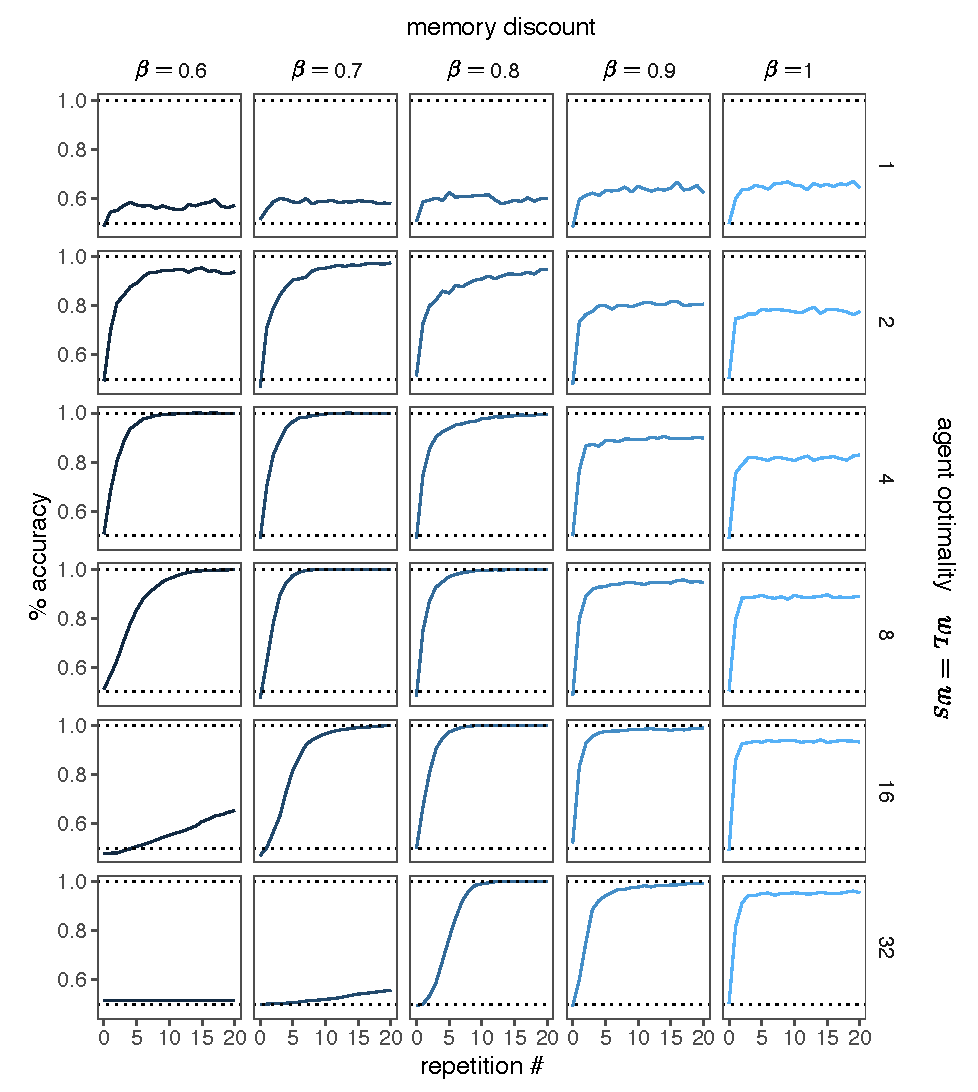
\includegraphics[scale=.9]{arbitrariness_grid.pdf}
  \caption{Coordination success (simulation 1.1) across a range of parameter values. Columns represent memory discount factors $\beta$, rows represent optimality parameters $w_S = w_L$. Communicative success is achieved under a wide range of settings, but convergence is limited in some regimes. At high values of $\beta$, with no ability to discount prior evidence, accuracy asymptotes quickly below perfect coordination; at low $\alpha$, inferences are weaker and agent actions are noisier, limiting the ability to converge; finally, at low values of $\beta$, when prior evidence is forgotten too quickly, convergence interacts with $\alpha$: when $\alpha$ is too high, the latest evidence may overwhelm all prior evidence, preventing the accumulation of shared history. The agent noise model is set to $\epsilon = 0.01$ in all simulations.}
  \label{fig:arbitrariness_grid}
\end{figure*}

 \begin{figure*}
\centering
    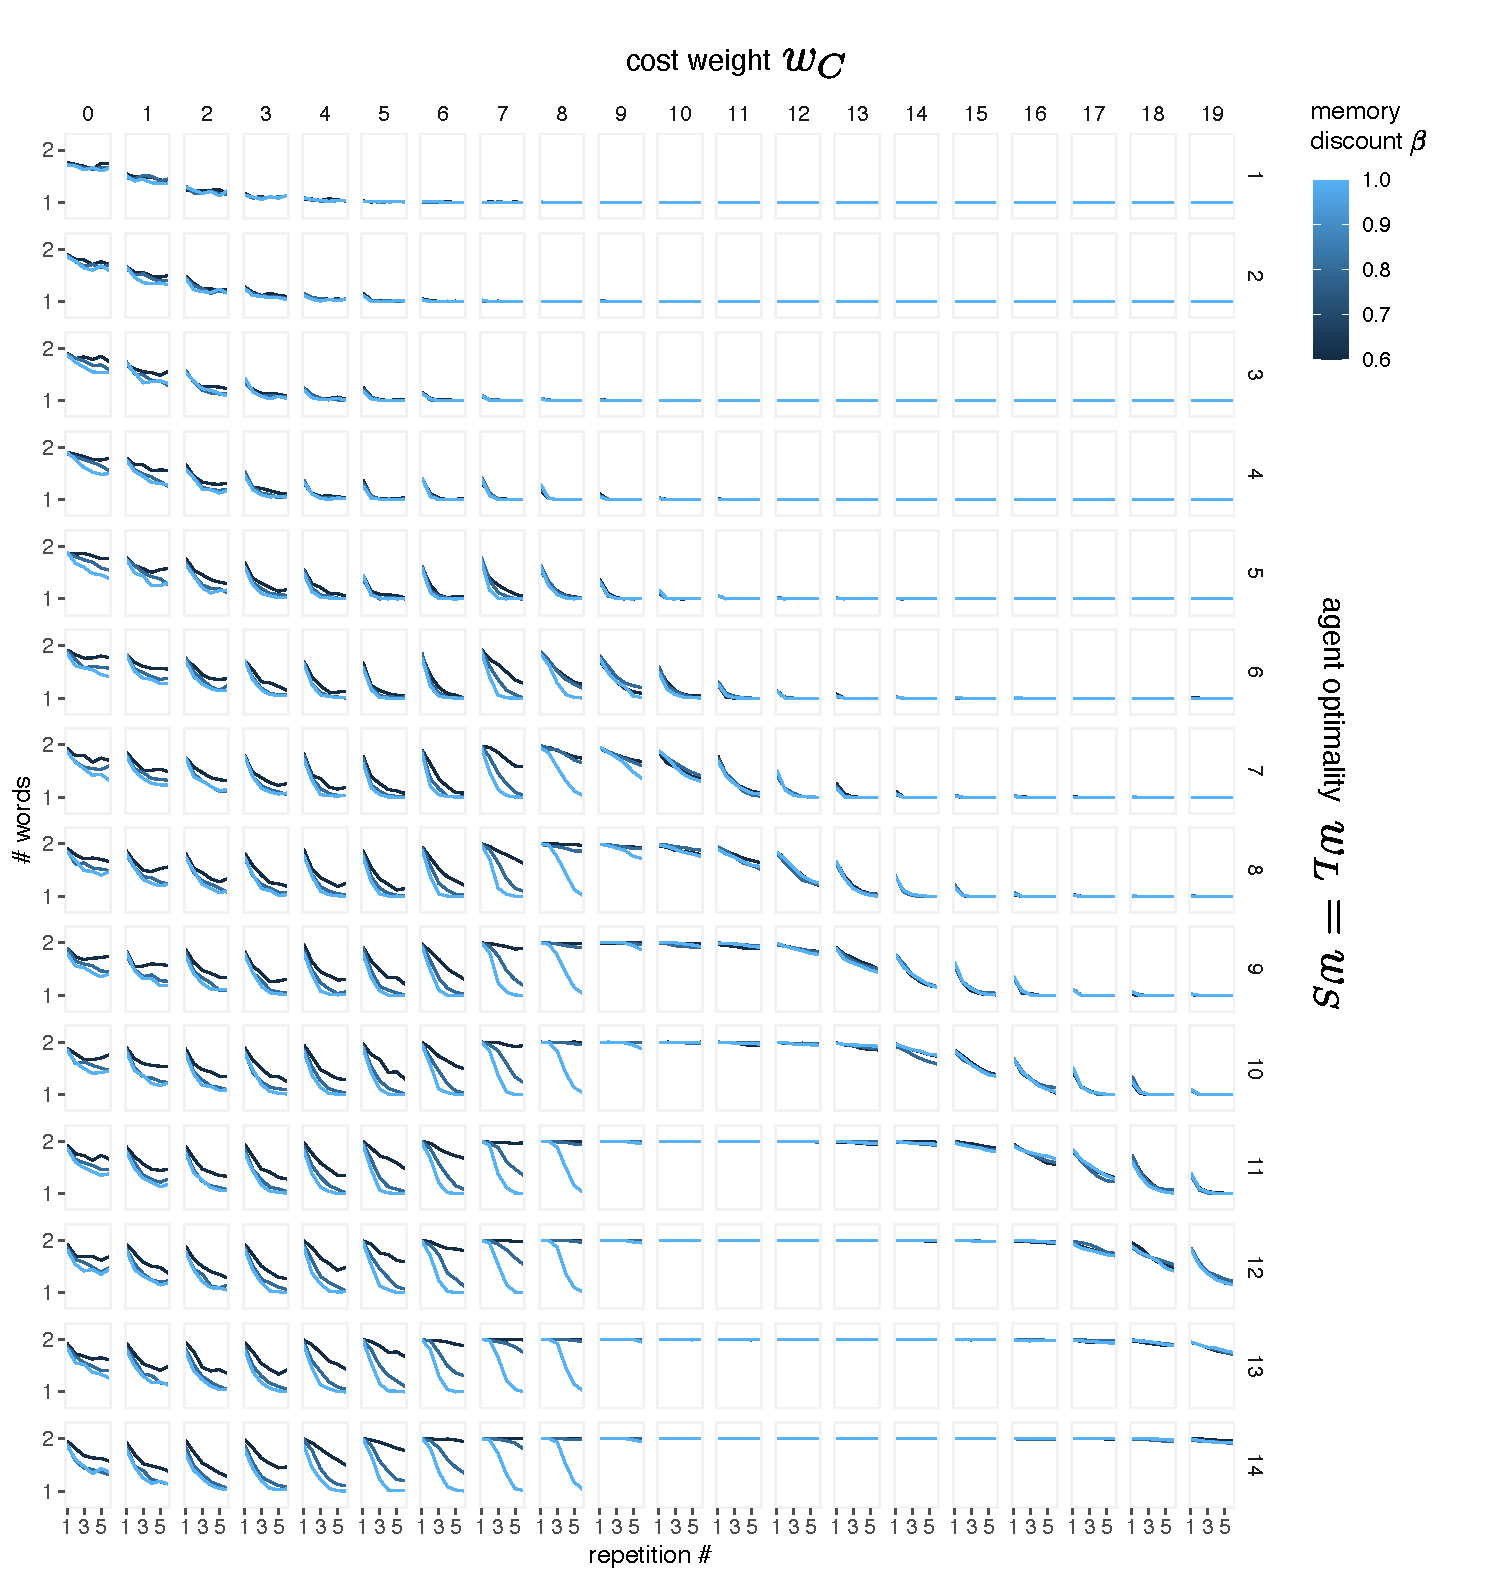
\includegraphics[scale=.7]{conjunction_grid.pdf}
  \caption{Speaker efficiency (simulation 1.2) across a range of parameter values representing different weights on informativity and cost. Rows represent agent optimality $w_S = w_L$, columns represent costs $w_C$, and different memory discount factors $\beta$ shown in different colors. Agents converge on more efficient ad hoc conventions for a wide regime of parameters. Broadly, when utterance cost is more heavily weighted relative to informativity, the speaker will not produce longer utterances even at the beginning of the interaction; when informativity is more heavily weighted, the speaker continues to prefer longer utterances despite their cost. Reduction is found at the critical point between this tradeoff. The exception is at low values of $w_C$, where reduction is found even at higher optimality simply due to compression when re-normalizing the speaker distribution.}
  \label{fig:conjunction_grid}
\end{figure*}

 \begin{figure*}
\centering
    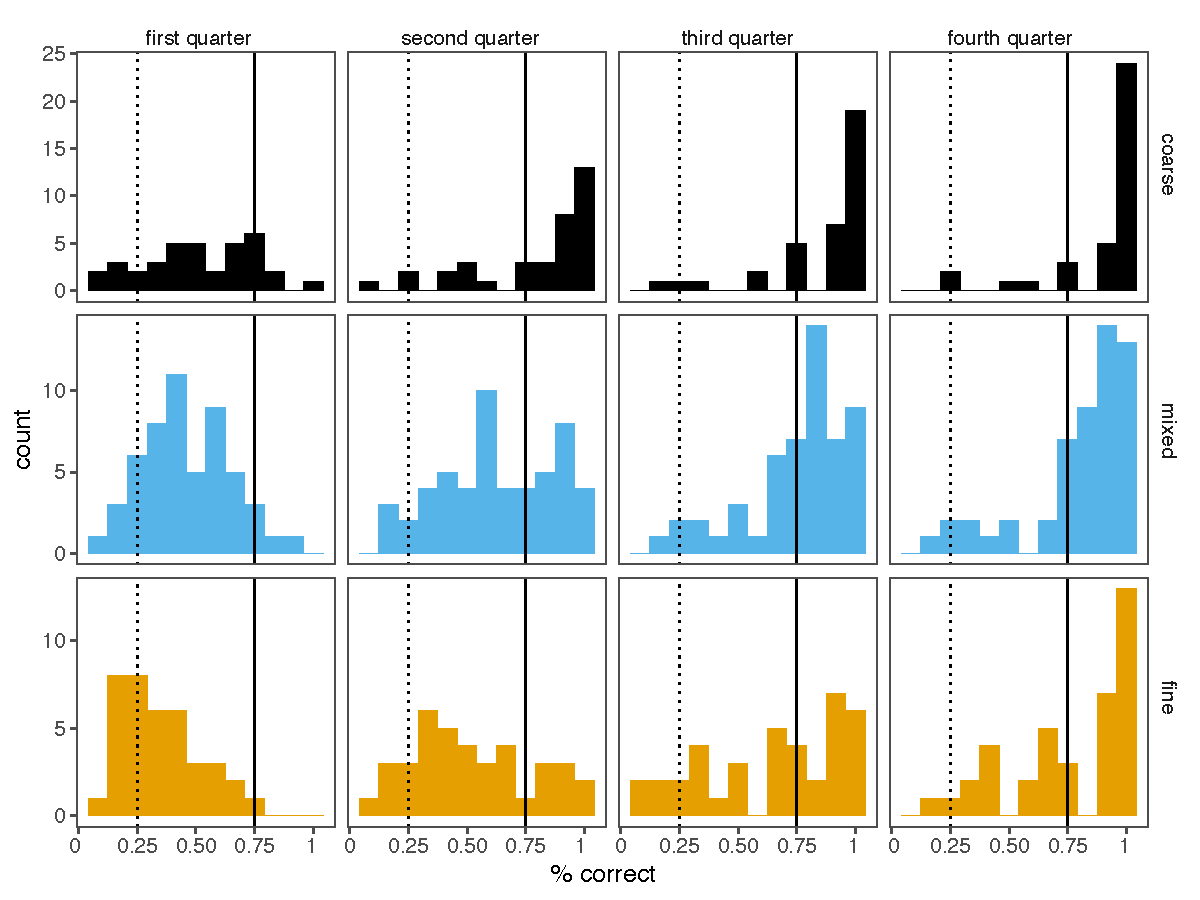
\includegraphics[scale=.9]{exp2-acc-grid_cleaned.pdf}
  \caption{Raw empirical accuracy distributions for context-sensitivity experiment. Each row represents how the accuracies of different games shift across the four quarters of the task for a given condition. Dotted vertical line represents chance accuracy (0.25), solid vertical line represents pre-registered convergence threshold (0.75).}
  \label{fig:full_accuracy_grid}
\end{figure*}

 \begin{figure*}
\centering
    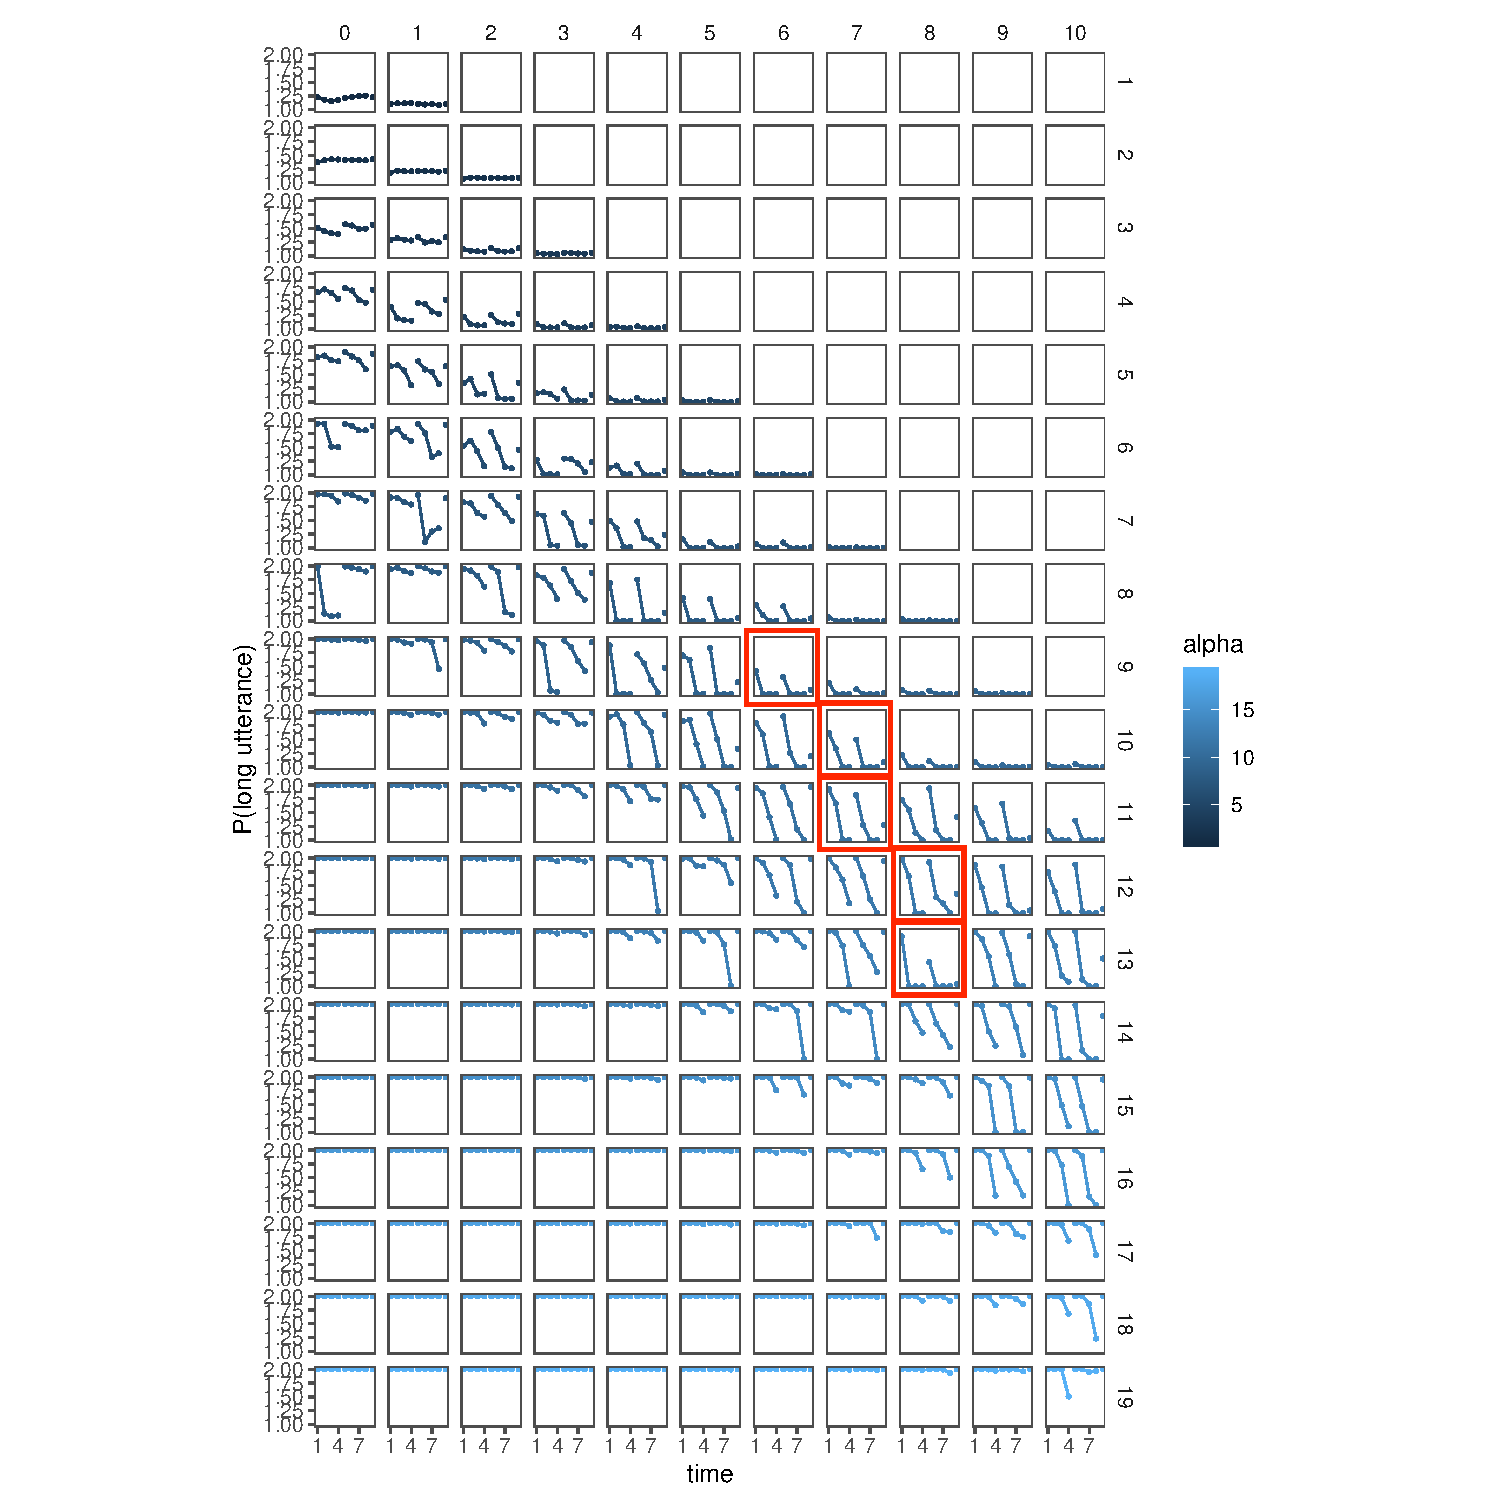
\includegraphics[scale=.8]{reduction_grid_search.pdf}
  \caption{Speaker efficiency across partners (simulation 3.2) for a range of parameter values. Rows represent speaker optimality $w_S$, columns represent cost weight $w_c$.}
  \label{fig:partnerspecificity_grid}
\end{figure*}
\end{document}  

